


\documentclass[a4paper]{article}\usepackage[]{graphicx}\usepackage[]{color}
%% maxwidth is the original width if it is less than linewidth
%% otherwise use linewidth (to make sure the graphics do not exceed the margin)
\makeatletter
\def\maxwidth{ %
  \ifdim\Gin@nat@width>\linewidth
    \linewidth
  \else
    \Gin@nat@width
  \fi
}
\makeatother

\definecolor{fgcolor}{rgb}{0.345, 0.345, 0.345}
\newcommand{\hlnum}[1]{\textcolor[rgb]{0.686,0.059,0.569}{#1}}%
\newcommand{\hlstr}[1]{\textcolor[rgb]{0.192,0.494,0.8}{#1}}%
\newcommand{\hlcom}[1]{\textcolor[rgb]{0.678,0.584,0.686}{\textit{#1}}}%
\newcommand{\hlopt}[1]{\textcolor[rgb]{0,0,0}{#1}}%
\newcommand{\hlstd}[1]{\textcolor[rgb]{0.345,0.345,0.345}{#1}}%
\newcommand{\hlkwa}[1]{\textcolor[rgb]{0.161,0.373,0.58}{\textbf{#1}}}%
\newcommand{\hlkwb}[1]{\textcolor[rgb]{0.69,0.353,0.396}{#1}}%
\newcommand{\hlkwc}[1]{\textcolor[rgb]{0.333,0.667,0.333}{#1}}%
\newcommand{\hlkwd}[1]{\textcolor[rgb]{0.737,0.353,0.396}{\textbf{#1}}}%
\let\hlipl\hlkwb

\usepackage{framed}
\makeatletter
\newenvironment{kframe}{%
 \def\at@end@of@kframe{}%
 \ifinner\ifhmode%
  \def\at@end@of@kframe{\end{minipage}}%
  \begin{minipage}{\columnwidth}%
 \fi\fi%
 \def\FrameCommand##1{\hskip\@totalleftmargin \hskip-\fboxsep
 \colorbox{shadecolor}{##1}\hskip-\fboxsep
     % There is no \\@totalrightmargin, so:
     \hskip-\linewidth \hskip-\@totalleftmargin \hskip\columnwidth}%
 \MakeFramed {\advance\hsize-\width
   \@totalleftmargin\z@ \linewidth\hsize
   \@setminipage}}%
 {\par\unskip\endMakeFramed%
 \at@end@of@kframe}
\makeatother

\definecolor{shadecolor}{rgb}{.97, .97, .97}
\definecolor{messagecolor}{rgb}{0, 0, 0}
\definecolor{warningcolor}{rgb}{1, 0, 1}
\definecolor{errorcolor}{rgb}{1, 0, 0}
\newenvironment{knitrout}{}{} % an empty environment to be redefined in TeX

\usepackage{alltt}

\usepackage{hyperref}
\usepackage{graphicx}
\usepackage{longtable}
\usepackage[utf8]{inputenc}
% \usepackage[spanish]{babel}
\usepackage{underscore}

\newcommand{\etal}{{\it et alt.}}
\newcommand{\R}{{\it R}}
\newcommand{\Rpackage}[1]{{\texttt{#1}}}
\newcommand{\Rcode}[1]{{\texttt{#1}}}
\newcommand{\Rfun}[1]{{\texttt{#1}}}

\title{Análisis de datos de microarrays con R y Bioconductor\\
Selección de genes diferencialmente expresados}

\author{Alex Sánchez}

\bibliographystyle{plain}
\IfFileExists{upquote.sty}{\usepackage{upquote}}{}
\begin{document}


\setkeys{Gin}{width=0.7\textwidth} % Sets default width for R-Sweave generated figures

\maketitle

\tableofcontents

\section{Introducción y objetivos}

Este documento presenta una solución al ejercicio de análisis de microarrays propuesto en la asignatura de \emph{Genómica Funcional y Análisis de Microarrays}. Su objetivo no es mostrar como realizar el mejor análisis de microarrays posible sino como hacerlo utilizando los conceptos y ejemplos proporcionados en las unidades dedicadas a este tema.

\subsection{Estructura del documento}

Típicamente un trabajo científico o técnico se organiza en varias partes: \emph{Introducción}, \emph{Material y Métodos}, \emph{Resultados} y \emph{Discusión}. Dado que el objetivo de este estudio es demostrar la aplicación de los métodos de análisis explicados en la asignatura esta estructura se relajará. Después de la introducción se realizará una breve descripción del proceso general y los métodos utilizados en cada paso. A continuación se presentarán los resultados obtenidos en cada fase del análisis. Finalmente se presentará una breve discusión sobre las posibles limitaciones encontradas.

\subsection{Objetivos}

El objetivo de este trabajo es realizar un análisis de datos de microarrays 
para encontrar genes diferencialmente expresados entre varios tipos de tumores de cancer de mama clasificados en tres grupos: apocrinos (APO), basales (BAS) y luminales (LUMI). 

Esta clasificación se basa en la resistencia de los tumores a los receptores de estrógenos y de andrógenos. 
\begin{itemize}
\item Los tumores clasificados como ``APO'' son negativos para los receptores de estrógenos (ER-) y positivos para los receptores de andrógenos (AR+).
\item  los clasificados como ``LUMI'' son (ER+) y (AR+) y
\item los clasificados como ``BAS'' son (ER-) y (AR-).
\end{itemize}

Es conveniente destacar que, de hecho, el objetivo de la práctica difiere del objetivo del artículo en que se basa. Mientras que el artículo se busca  \emph{descubrir} los tres grupos con los que trabajamos en este ejercicio se pretende caracterizarlos a través de los gene que se expresan de forma distinta entre ellos. No deja de ser un problema del tipo ``el huevo y la gallina'', es decir: \emph{¿Puesto que se trata de grupos distintos encontramos genes que se expresan diferencialmente entre ellos o dado que hay genes que se expresan diferencialmente podemos deducir que son grupos distintos?}

\section{Materiales y métodos}

\subsection{Etapas del analisis}

El análisis se ha realizado siguiendo las pautas descritas en los capítulos 6 a 11 de los apuntes de la asignatura \url{http://ueb.vhir.org/cursos/Microarrays} y resumidos en la figura \ref{fig:pipeline}.

\begin{figure}[htbp]\begin{center}
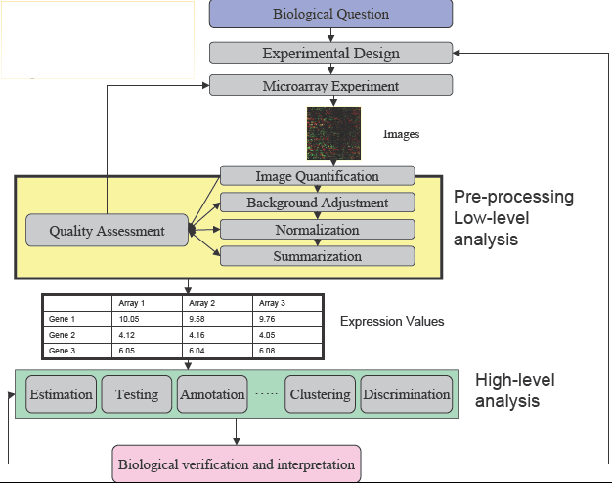
\includegraphics[width=9cm]{images/analysisProcess}\\
\caption{The Microarray Analysis Process}\label{fig:pipeline}
\end{center}
\end{figure}

\subsection{Métodos de análisis}

Antes de hibridar los microarrays\footnote{Esta primera parte es ficticia en tanto que no hemos tendio acceso al proceso de elaboración de los microarrays, por lo que he escrito lo que suele ponerse en esta parte} se comprobó la calidad del cRNA de cada muestra. Sólo las que demostraron una calidad suficiente --presumiblemente un valor de ``Bio-analyser''\footnote{Sistema para el análisi de la calidad del RNA} igual o superior a 7-- se sometieron a análisis posterior.. 

Los valores ``crudos'' de expresión obtenidos directamente de los archivos CEL se preprocesa utilizando el método de RMA (\cite{Irizarry:2003}), un proceso de tres pasos que integra la corrección de fondo, la normalización y el resumen de los valores del grupo de sondas en un único valor de expresión ``absoluta''. Dichos valores normalizados fueron la base para todos los análisis.

Antes de la selección de genes los valores normalizados se sometieron a un filtraje no específico para eliminar los genes de baja 
%señal (los genes cuya media de la señal en cada grupo no supera un umbral mínimo) y los genes de baja 
variabilidad (los genes cuyo rango intercuartil entre todas las muestras no superó un umbral mínimo).

La selección de genes diferencialmente expresados entre condiciones experimentales se basó en el método desarrollado por Smyth y otros ~\cite{Smyth:2004}.

%La selecci\'on de genes ​diferencialmente expresados entre condiciones experimentales se bas\'o en la utilización de modelos lineales complementados con una moderación de la varianza mediante m\'etodos bayesianos emp\'iricos siguiendo la metodolog\'ia desarrollada por Smyth \cite{Smyth:2004}.

Este método extiende el análisis de la varianza clásico utilizando métodos Bayesianos empíricos para combinar la información de cada gen individual con la de todos los genes restantes para obtener mejores estimaciones de error. Esto es de gran utilidad en análisis de microarrays, un contexto en el que el tamaño de las muestras es a menudo pequeño lo que puede dar lugar a estimaciones de los errores erráticos y, en consecuencia, p--valores que no son de fiar.

Los genes más relevantes de cada comparaci\'on se resaltaron utilizando ``volcano-plots'', 
que organizan los genes a lo largo de dos dimensiones que podemos considerar de importancia biológica y estadística. El eje horizontal representa el cambio medio de expresión entre los dos grupos (en una escala logarítmica, por lo que la regulación hacia arriba y abajo aparecen simétrica), y el segundo (vertical) representa el ``menos logaritmo del p-valor'' por lo que los genes cuyo p-valor asociado sea inferior aparecen más arriba. El primer eje indica el impacto biológico del cambio, y el segundo indica la evidencia estadística, o la fiabilidad de dicho cambio.


Con el fin de hacer frente a la problemática derivada del hecho de que muchas pruebas (una por cada gen) se realizan simultáneamente, se realizo un ajuste de p--valores para obtener control sobre la tasa de falsos positivos usando el método de Benjamini y Hochberg (\cite{BenjaminiHochberg:1995}).



Los genes seleccionados como diferencialmente expresados se agruparon para buscar patrones comunes de expresión entre condiciones experimentales.
Para ello se utilizaron mapas de colores o ``Heatmaps'' que realizan una agrupación jerárquica de los genes y/o las muestras y la representan mediante una gama de colores apropiada, de forma que valores altos o bajos se corresponden a colores distintos de la gama escogida.

Las listas de genes diferencialmente expresados se anotaron en diversas bases de datos (Entrez, Unigene, Gene Ontology, KEGG, ...) utilizando los paquetes de anotación para microarrays de affymetrix disponibles en el proyecto Bioconductor (\url{http://bioconductor.org}).

Para contribuir a la interpretación biológica de los resultados se realizó un análisis de enriquecimiento \cite{Gentleman:2004, Falcon:2007} que busca establecer si las categorias funcionales de los genes seleccionados aparecen entre estos genes con mayor (o menor) frecuencia que entre todos los del genoma. De ser así se indica que la lista de genes se encuentra ``enriquecida'' en estas funcionalidades, o lo que es lo mismo que los procesos afectados por las diferencias son éstos.

\subsubsection{Herramientas y procedimientos  bioinformáticos de análisis}

Los análisis estadísticos se realizaron utilizando el lenguaje estadístico  \R  y las librerías  desarrolladas para el análisis de microarray en el proyecto de Bioconductor (\url{www.bioconductor.org}). Para más detalle sobre los métodos descritos en esta sección puede consultarse \cite{Gentleman:2005}.

El código siguiente se utilizó para instalar los paquetes de Bioconductor necesarios para el análisis.

\begin{knitrout}
\definecolor{shadecolor}{rgb}{0.969, 0.969, 0.969}\color{fgcolor}\begin{kframe}
\begin{verbatim}
## [1] "Package Biobase already installed"
## [1] "Package affy already installed"
## [1] "Package arrayQualityMetrics already installed"
## [1] "Package genefilter already installed"
## [1] "Package multtest already installed"
\end{verbatim}


{\ttfamily\noindent\color{warningcolor}{\#\# Warning: package 'limma' was built under R version 3.3.3}}\begin{verbatim}
## [1] "Package limma already installed"
\end{verbatim}


{\ttfamily\noindent\color{warningcolor}{\#\# Warning: package 'IRanges' was built under R version 3.3.3}}

{\ttfamily\noindent\color{warningcolor}{\#\# Warning: package 'S4Vectors' was built under R version 3.3.3}}\begin{verbatim}
## [1] "Package hgu133a.db already installed"
\end{verbatim}


{\ttfamily\noindent\color{warningcolor}{\#\# Warning: package 'XML' was built under R version 3.3.3}}\begin{verbatim}
## [1] "Package annotate already installed"
## [1] "Package annaffy already installed"
## [1] "Package hwriter already installed"
\end{verbatim}


{\ttfamily\noindent\color{warningcolor}{\#\# Warning: package 'gplots' was built under R version 3.3.3}}\begin{verbatim}
## [1] "Package gplots already installed"
## [1] "Package GOstats already installed"
## [1] "Package GSA already installed"
\end{verbatim}
\end{kframe}
\end{knitrout}


\section{Obtención y lectura de los datos}

\subsection{Los datos para el análisis}

Los datos en que se basa el estudio se han obtenido a partir de tumores de mama (``advanced/inflammatory breast tumours'') y fueron tomados antes del tratamiento de pacientes enrolados en un estudio clínico (EORTC 10994). 

Los microarrays se prepararon a partir de RNA total extraído de secciones de 25 mm de biopsias y amplificados mediante el procedimiento ``Eberwine T7 procedure'' siguiendo el protocolo indicado por Affymetrix para pequeñas muestras.

Los datos de los microarrays se encuentran en Gene Expression Omnibus (GEO) con el número de serie GSE1561. Puede accederse a ellos  en el siguiente enlace \url{http://www.ncbi.nlm.nih.gov/geo/query/acc.cgi?acc=GSE1561}. El artículo de Farmer (\cite{Farmer2005}) \etal (\url{http://www.ncbi.nlm.nih.gov/pubmed/15897907}) describe el estudio.

\subsubsection{Localización de los datos}

Como es habitual en este curso supondremos que trabajamos en un directorio 
escogido por nosotros y cuya localización se asigna a la variable \texttt{workingDir}.

Asumiremos que los datos se encuentran en un subdirectorio del anterior, denominado ``data'' que se almacenará en la variable \texttt{dataDir} y que los resultados se almacenarán en un directorio ``results'' cuyo nombre completo se almacenará en la variable  \texttt{resultsDir}.

\begin{knitrout}
\definecolor{shadecolor}{rgb}{0.969, 0.969, 0.969}\color{fgcolor}\begin{kframe}
\begin{alltt}
\hlstd{workingDir} \hlkwb{<-}\hlkwd{getwd}\hlstd{()}
\hlstd{dataDir} \hlkwb{<-}\hlkwd{file.path}\hlstd{(workingDir,} \hlstr{"data"}\hlstd{)}
\hlstd{resultsDir} \hlkwb{<-} \hlkwd{file.path}\hlstd{(workingDir,}\hlstr{"results"}\hlstd{)}
\hlstd{celfilesDir} \hlkwb{<-} \hlkwd{file.path}\hlstd{(workingDir,}\hlstr{"celfiles"}\hlstd{)}
\hlkwd{setwd}\hlstd{(workingDir)}
\end{alltt}
\end{kframe}
\end{knitrout}

\subsubsection{Selección de muestras para el análisis}

Este análisis se ha basado en un subconjunto de muestras del estudio original.
Las muestras se han obtenido de la lista original mediante un pequeño script de \R.

De la dirección  \url{http://www.ncbi.nlm.nih.gov/geo/query/acc.cgi?acc=GSE1561}  es posible descargar un archivo comprimido con los 49 archivos ``.cel''. Con el fin de simplificar el análisis se decidió seleccionar aleatoriamente 5 arrays de cada grupo utilizando a partir de la información contenida en el archivo: ``Asignacion_de_Muestras_A_Grupos.csv'' elaborado a partir de la información sobre el diseño experimental contenida en: \url{http://www.ncbi.nlm.nih.gov/geo/gds/profileGraph.cgi?gds=1329}

\begin{knitrout}
\definecolor{shadecolor}{rgb}{0.969, 0.969, 0.969}\color{fgcolor}\begin{kframe}
\begin{alltt}
\hlcom{# muestras <- read.csv2(file.path(dataDir, "Asignacion_de_muestras_a_grupos.csv"),  head=T)}
\hlcom{# misMuestras <- as.character (muestras$Sample)}
\hlcom{# paraAnalisis <- c(sample(misMuestras[1:6], 5), }
\hlcom{#                  sample(misMuestras[7:20], 5),}
\hlcom{#                  sample(misMuestras[23:48], 5))}
\hlcom{# alAnalisis <-muestras[muestras$Sample %in% paraAnalisis,]}
\hlcom{# write.table(alAnalisis, file=file.path(dataDir, "targets.txt"), }
\hlcom{#            sep="\textbackslash{}t", row.names=FALSE, quote=FALSE)}
\end{alltt}
\end{kframe}
\end{knitrout}

\subsubsection{Lectura de los datos}

La lectura de datos se lleva a cabo utilizando las clases y métodos definidas en los paquetes \Rcode{Biobase} y \Rcode{affy} de Bioconductor.

Una forma cómoda de leer los datos y, al mismo tiempo, asignar a cada muestra los valores de las covariables (por ejemplo el grupo para el analisis) consiste en crear un pequeño archivo de texto, que suele denominarse \Rcode{targets.txt} y que contiene la identificacion de cada archivo con la asignación de cada muestra a cada condición experimental. El archivo targets para este caso tiene el aspecto que se muestra en la tabla siguiente.

\begin{kframe}


{\ttfamily\noindent\itshape\color{messagecolor}{\#\# Loading required package: xtable}}\end{kframe}% latex table generated in R 3.3.2 by xtable 1.8-2 package
% Wed May 24 00:33:25 2017
\begin{longtable}{rllll}
  \hline
 & Sample & Ids & SampleIDs & Group \\ 
  \hline
GSM26878.CEL & GSM26878 & PF14 EnPnT2N1G2 & PF14 & A \\ 
  GSM26883.CEL & GSM26883 & PF19 EnPuT4N0Gu & PF19 & A \\ 
  GSM26887.CEL & GSM26887 & PF23 EnPnT2N0G2 & PF23 & A \\ 
  GSM26903.CEL & GSM26903 & PF39 EnPuT4N0Gu & PF39 & A \\ 
  GSM26910.CEL & GSM26910 & PF46 EnPnT4N1G3 & PF46 & A \\ 
  GSM26888.CEL & GSM26888 & PF24 EnPnTiN0G3 & PF24 & B \\ 
  GSM26889.CEL & GSM26889 & PF25 EnPnT3N2G2 & PF25 & B \\ 
  GSM26892.CEL & GSM26892 & PF28 EnPnT2N1G3 & PF28 & B \\ 
  GSM26898.CEL & GSM26898 & PF34 EnPnT3N1G3 & PF34 & B \\ 
  GSM26906.CEL & GSM26906 & PF42 EnPnT2N2G3 & PF42 & B \\ 
  GSM26879.CEL & GSM26879 & PF15 EpPnTiN1G3 & PF15 & L \\ 
  GSM26896.CEL & GSM26896 & PF32 EpPnT3N1G2 & PF32 & L \\ 
  GSM26897.CEL & GSM26897 & PF33 EpPnTiN0G2 & PF33 & L \\ 
  GSM26907.CEL & GSM26907 & PF43 EpPpT2N1G2 & PF43 & L \\ 
  GSM26911.CEL & GSM26911 & PF47 EpPpT3N1G3 & PF47 & L \\ 
   \hline
\hline
\caption{Archivo targets.txt con la asignación a cada muestra de su condición experimental} 
\end{longtable}


El contenido del archivo \texttt{targets} se utiliza en la lectura de los datos y la creación del objeto \texttt{rawData} de la clase \texttt{affybatch} que contendrá las intensidade ``crudas'' de cada archivo .CEL

\begin{knitrout}
\definecolor{shadecolor}{rgb}{0.969, 0.969, 0.969}\color{fgcolor}\begin{kframe}
\begin{alltt}
\hlkwd{require}\hlstd{(affy)}
\hlstd{sampleInfo} \hlkwb{<-} \hlkwd{read.AnnotatedDataFrame}\hlstd{(}\hlkwd{file.path}\hlstd{(dataDir,}\hlstr{"targets.txt"}\hlstd{),}
    \hlkwc{header} \hlstd{=} \hlnum{TRUE}\hlstd{,} \hlkwc{row.names} \hlstd{=} \hlnum{1}\hlstd{,} \hlkwc{sep}\hlstd{=}\hlstr{"\textbackslash{}t"}\hlstd{)}
\hlstd{fileNames} \hlkwb{<-} \hlkwd{rownames}\hlstd{(}\hlkwd{pData}\hlstd{(sampleInfo))}
\hlstd{rawData} \hlkwb{<-} \hlkwd{read.affybatch}\hlstd{(}\hlkwc{filenames}\hlstd{=}\hlkwd{file.path}\hlstd{(celfilesDir,fileNames),}
                          \hlkwc{phenoData}\hlstd{=sampleInfo)}
\hlkwd{show}\hlstd{(rawData)}
\end{alltt}


{\ttfamily\noindent\color{warningcolor}{\#\# Warning: replacing previous import 'AnnotationDbi::tail' by 'utils::tail' when loading 'hgu133acdf'}}

{\ttfamily\noindent\color{warningcolor}{\#\# Warning: replacing previous import 'AnnotationDbi::head' by 'utils::head' when loading 'hgu133acdf'}}

{\ttfamily\noindent\itshape\color{messagecolor}{\#\# }}\begin{verbatim}
## AffyBatch object
## size of arrays=712x712 features (27 kb)
## cdf=HG-U133A (22283 affyids)
## number of samples=15
## number of genes=22283
## annotation=hgu133a
## notes=
\end{verbatim}
\end{kframe}
\end{knitrout}

Este objeto es la base para todos los análisis que se realizarán.


\section{Preprocesado: Exploración, Control de Calidad y Normalización}

Los datos procedentes de la lectura de los microarrays se denominan datos ``crudos'' y deben ser pre-procesados de diversas formas antes de analizarlos.

``Preprocesado'' es un término genérico que engloba varios procesos
\begin{itemize}
\item Exploración y control de calidad de los datos.
\item Normalización y resumen (llamdo ``sumarización'') de los valores de las sondas de cada grupo de sondas.
\item Filtrado no específico para eliminar el efecto de genes que no se expresan o bien no se expresan de forma distinta entre los grupos.
\end{itemize}

A su vez la exploración y el control de calidad contempla:
\begin{enumerate}
\item Exploraciones estadísticas estándar.
\item Técnicas de control de calidad desarrolladas específicamente para datos de microarrays.
\end{enumerate}

\subsection{Exploración y visualización}

La exploración de los datos suele basarse en técnicas univariantes
como los histogramas o los diagramas de caja o en técnicas
multivariantes como los análisis de conglomerados (``clusters''), de
distancias o de análisis de componentes principales.

\subsubsection{Exploración estadística de los datos}



Un gráfico de densidad --mal llamado en este contexto, histograma--
permite hacerse una idea de si las distribuciones de los distintos
arrays son similares en forma y posición.

\begin{figure}[htbp]
\begin{knitrout}
\definecolor{shadecolor}{rgb}{0.969, 0.969, 0.969}\color{fgcolor}
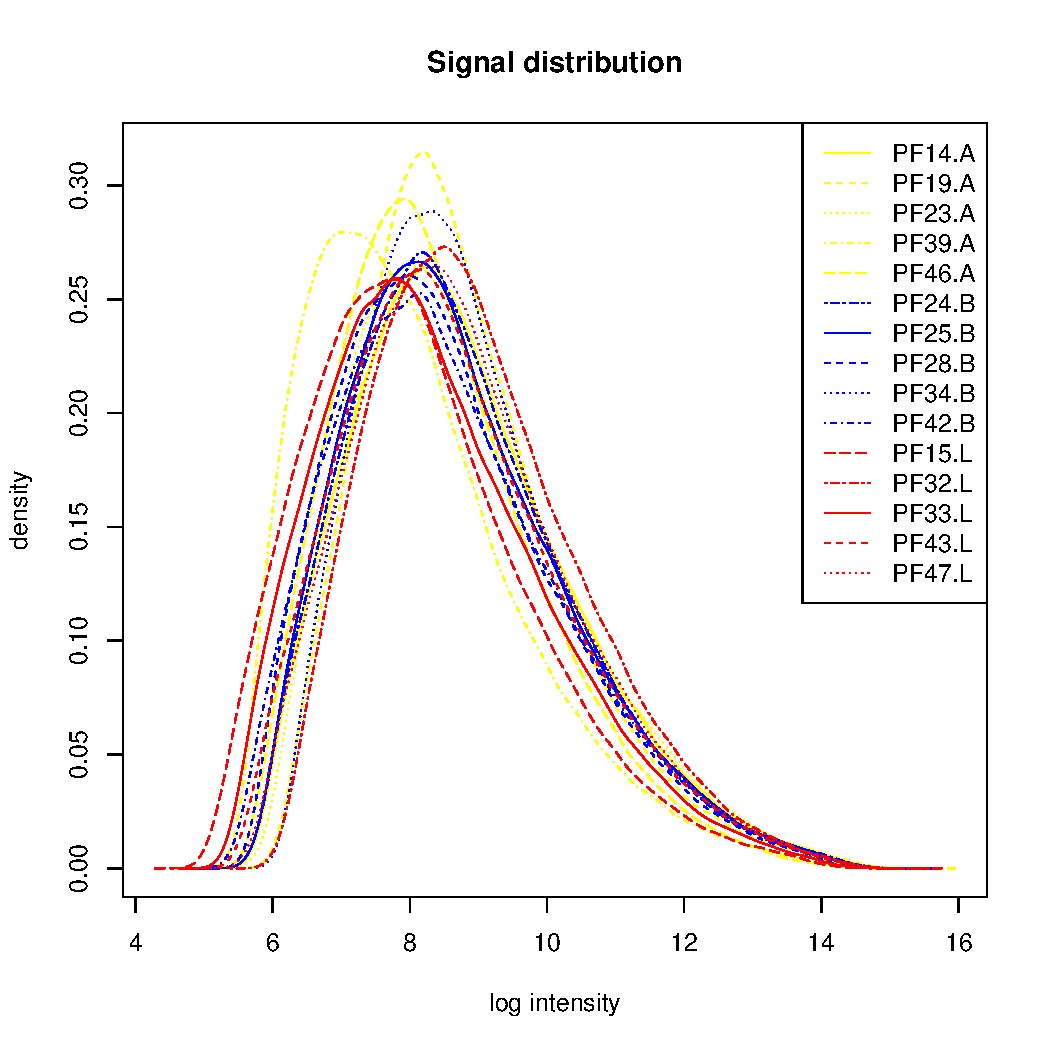
\includegraphics[width=\maxwidth]{images/graficplotHist-1} 

\end{knitrout}
\caption{Distribución de las expresiones de cada array. Aunque los gráficos muestran una cierta heterogeneidad entre muestras el aspecto de todas ellas es compatible con la "normalidad" es decir no sugieren que pueda haber algún problema en los datos.}
\end{figure}

Un diagrama de cajas muestra la misma información facilitando más la comparaci\'on entre distribuciones.
  
\begin{figure}[htbp]
\centering
\begin{knitrout}
\definecolor{shadecolor}{rgb}{0.969, 0.969, 0.969}\color{fgcolor}\begin{kframe}
\begin{alltt}
\hlkwd{boxplot}\hlstd{(rawData,} \hlkwc{cex.axis}\hlstd{=}\hlnum{0.6}\hlstd{,} \hlkwc{col}\hlstd{=colores,} \hlkwc{las}\hlstd{=}\hlnum{2}\hlstd{,} \hlkwc{names}\hlstd{=sampleNames,}
        \hlkwc{main}\hlstd{=}\hlstr{"Signal distribution for selected chips"}\hlstd{)}
\end{alltt}
\end{kframe}
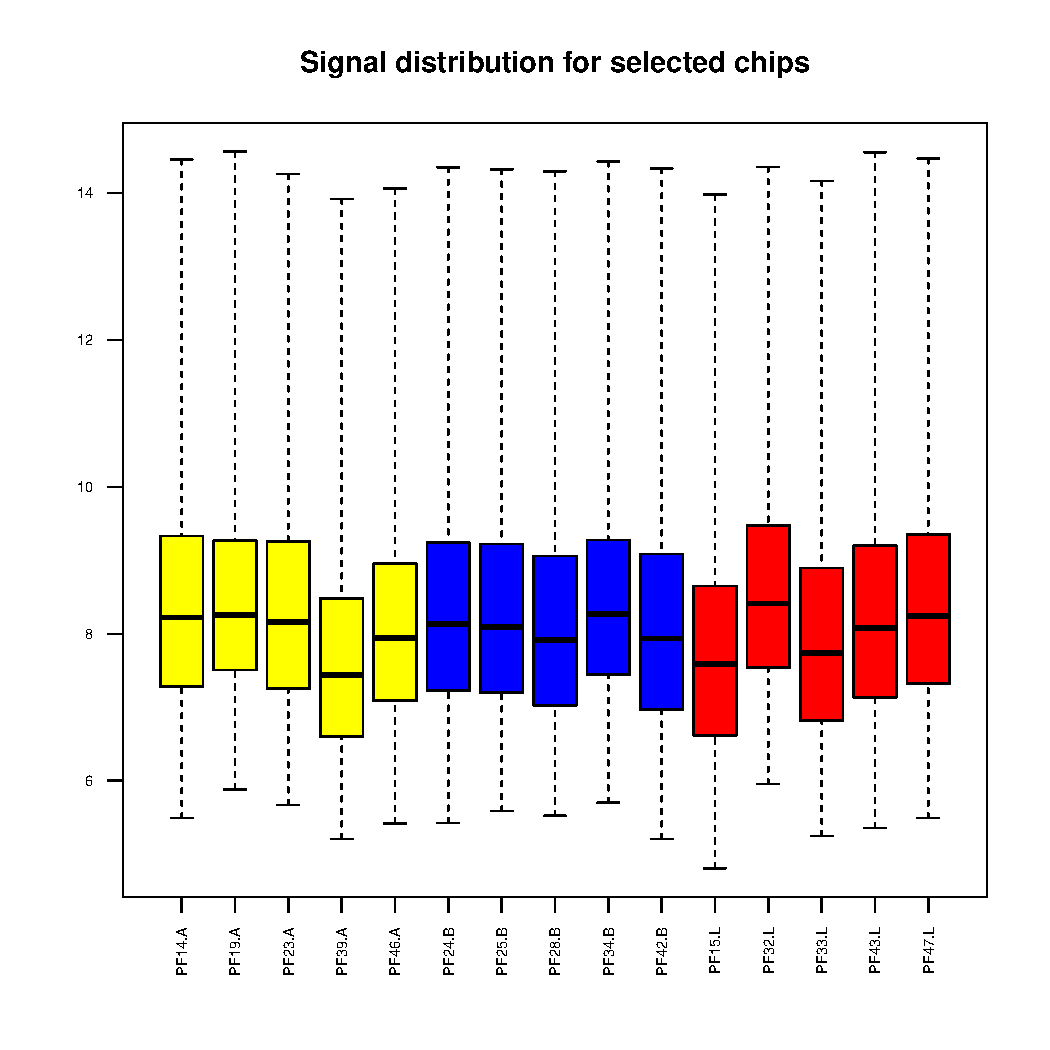
\includegraphics[width=\maxwidth]{images/graficboxplot-1} 

\end{knitrout}
  \caption{El diagrama de cajas muestra, de forma similar al histograma, cómo las distribuciones de los datos son relativamente similares. Hay heterogeneidad pero no se muestra ninguna diferencia sistemática, lo que sugiere que es conveniente normalizar peró no parece que hayan arrays problemáticos}
  \label{fig:boxplot}
\end{figure}

Una representación multivariante como la ofrecida por los gráficos de las componentes principales suele resultar muy informativa de posibles problemas como efectos batch o presencia de valores "raros". El gráfico de componentes principales muestra los datos en dimensión reducida de forma que cada componente explica una dimensión de mayor variabilidad e independiente de la siguiente. Representando el porcentaje de variabilidad explicada para cada componente tenemos una medida de la importancia de los grupos que se puedan visualizar. Si la suma de los porecentajes es alta, por ejemplo superior al 50\% las conclusiones que de ellos se deriven seran más fiables que con valores bajos, por ejemplo inferiores al 30\% de varianza explicada.

\begin{knitrout}
\definecolor{shadecolor}{rgb}{0.969, 0.969, 0.969}\color{fgcolor}\begin{kframe}
\begin{alltt}
\hlstd{plotPCA} \hlkwb{<-} \hlkwa{function} \hlstd{(} \hlkwc{X}\hlstd{,} \hlkwc{labels}\hlstd{=}\hlkwa{NULL}\hlstd{,} \hlkwc{colors}\hlstd{=}\hlkwa{NULL}\hlstd{,} \hlkwc{dataDesc}\hlstd{=}\hlstr{""}\hlstd{,} \hlkwc{scale}\hlstd{=}\hlnum{FALSE}\hlstd{)}
\hlstd{\{}
  \hlstd{pcX}\hlkwb{<-}\hlkwd{prcomp}\hlstd{(}\hlkwd{t}\hlstd{(X),} \hlkwc{scale}\hlstd{=scale)} \hlcom{# o prcomp(t(X))}
  \hlstd{loads}\hlkwb{<-} \hlkwd{round}\hlstd{(pcX}\hlopt{$}\hlstd{sdev}\hlopt{^}\hlnum{2}\hlopt{/}\hlkwd{sum}\hlstd{(pcX}\hlopt{$}\hlstd{sdev}\hlopt{^}\hlnum{2}\hlstd{)}\hlopt{*}\hlnum{100}\hlstd{,}\hlnum{1}\hlstd{)}
  \hlstd{xlab}\hlkwb{<-}\hlkwd{c}\hlstd{(}\hlkwd{paste}\hlstd{(}\hlstr{"PC1"}\hlstd{,loads[}\hlnum{1}\hlstd{],}\hlstr{"%"}\hlstd{))}
  \hlstd{ylab}\hlkwb{<-}\hlkwd{c}\hlstd{(}\hlkwd{paste}\hlstd{(}\hlstr{"PC2"}\hlstd{,loads[}\hlnum{2}\hlstd{],}\hlstr{"%"}\hlstd{))}
  \hlkwa{if} \hlstd{(}\hlkwd{is.null}\hlstd{(colors)) colors}\hlkwb{=}\hlnum{1}
  \hlkwd{plot}\hlstd{(pcX}\hlopt{$}\hlstd{x[,}\hlnum{1}\hlopt{:}\hlnum{2}\hlstd{],}\hlkwc{xlab}\hlstd{=xlab,}\hlkwc{ylab}\hlstd{=ylab,} \hlkwc{col}\hlstd{=colors,}
       \hlkwc{xlim}\hlstd{=}\hlkwd{c}\hlstd{(}\hlkwd{min}\hlstd{(pcX}\hlopt{$}\hlstd{x[,}\hlnum{1}\hlstd{])}\hlopt{-}\hlnum{10}\hlstd{,} \hlkwd{max}\hlstd{(pcX}\hlopt{$}\hlstd{x[,}\hlnum{1}\hlstd{])}\hlopt{+}\hlnum{10}\hlstd{))}
  \hlkwd{text}\hlstd{(pcX}\hlopt{$}\hlstd{x[,}\hlnum{1}\hlstd{],pcX}\hlopt{$}\hlstd{x[,}\hlnum{2}\hlstd{], labels,} \hlkwc{pos}\hlstd{=}\hlnum{3}\hlstd{,} \hlkwc{cex}\hlstd{=}\hlnum{0.8}\hlstd{)}
  \hlkwd{title}\hlstd{(}\hlkwd{paste}\hlstd{(}\hlstr{"Plot of first 2 PCs for expressions in"}\hlstd{, dataDesc,} \hlkwc{sep}\hlstd{=}\hlstr{" "}\hlstd{),} \hlkwc{cex}\hlstd{=}\hlnum{0.8}\hlstd{)}
\hlstd{\}}
\end{alltt}
\end{kframe}
\end{knitrout}

\begin{figure}[htbp]
\centering
\begin{knitrout}
\definecolor{shadecolor}{rgb}{0.969, 0.969, 0.969}\color{fgcolor}\begin{kframe}
\begin{alltt}
\hlkwd{plotPCA}\hlstd{(}\hlkwd{exprs}\hlstd{(rawData),} \hlkwc{labels}\hlstd{=sampleNames,} \hlkwc{dataDesc}\hlstd{=}\hlstr{"selected samples"}\hlstd{)}
\end{alltt}
\end{kframe}
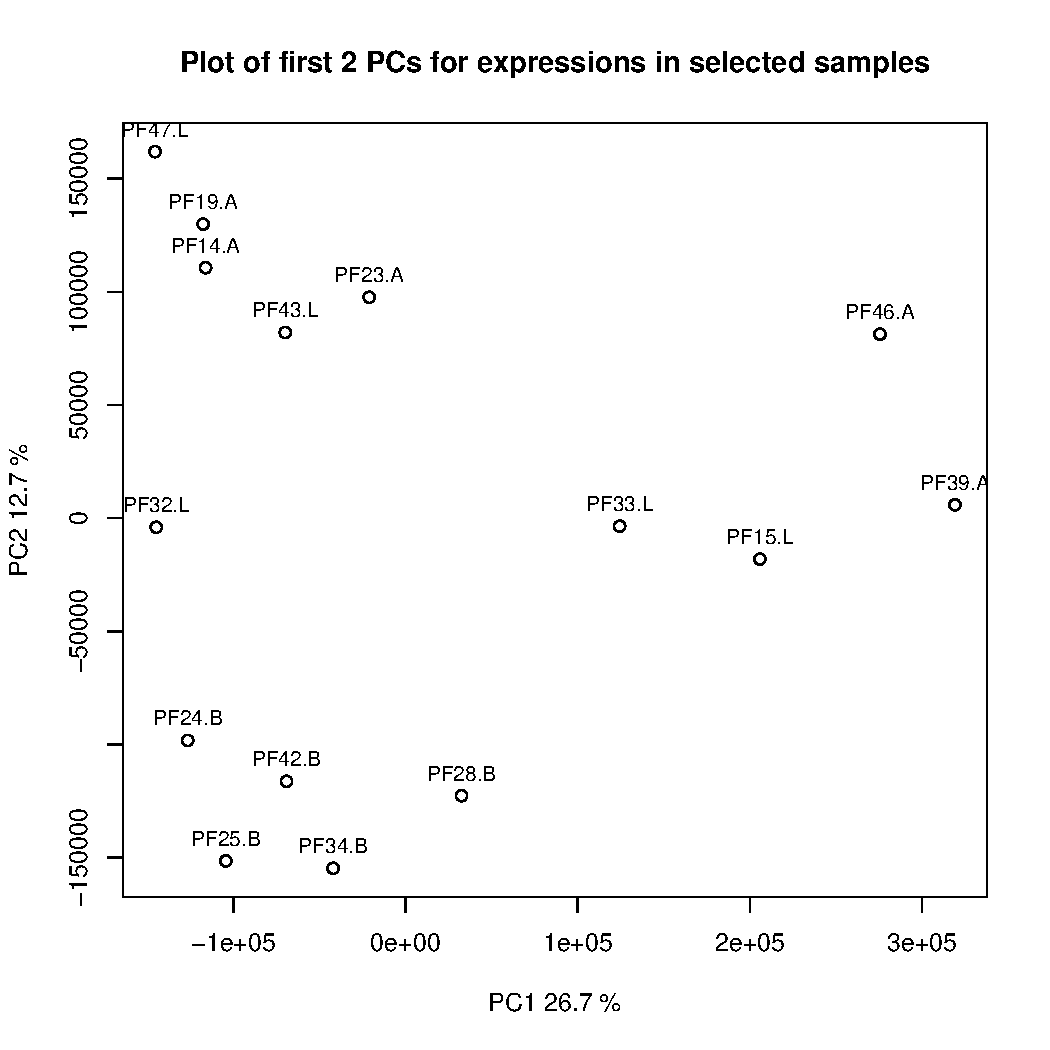
\includegraphics[width=\maxwidth]{images/graficplotPCA2D-1} 

\end{knitrout}
\caption{Representación de las dos primeras componentes de un análisi de components principales. Los grupos aparecen algo separados pero el porcentaje de variabilidad explicado por las dos primeras componentes sugiere que puede no ser muy explicativas}
\label{fig:PCA2D}
\end{figure}

Un enfoque alternativo al del PCA aunque relacionado es realizar un análisis basado en distancias. Podemos hacerlo calculando y visualizando la matriz de distancias mediante un mapa de colores o mediante un agrupamiento jerárquico seguido de un dendrograma.

\begin{figure}
\centering
\begin{knitrout}
\definecolor{shadecolor}{rgb}{0.969, 0.969, 0.969}\color{fgcolor}\begin{kframe}
\begin{alltt}
  \hlstd{manDist} \hlkwb{<-}  \hlkwd{dist}\hlstd{(}\hlkwd{t}\hlstd{(}\hlkwd{exprs}\hlstd{(rawData)))}
  \hlkwd{heatmap} \hlstd{(}\hlkwd{as.matrix}\hlstd{(manDist),}  \hlkwc{col}\hlstd{=}\hlkwd{heat.colors}\hlstd{(}\hlnum{16}\hlstd{))}
\end{alltt}
\end{kframe}
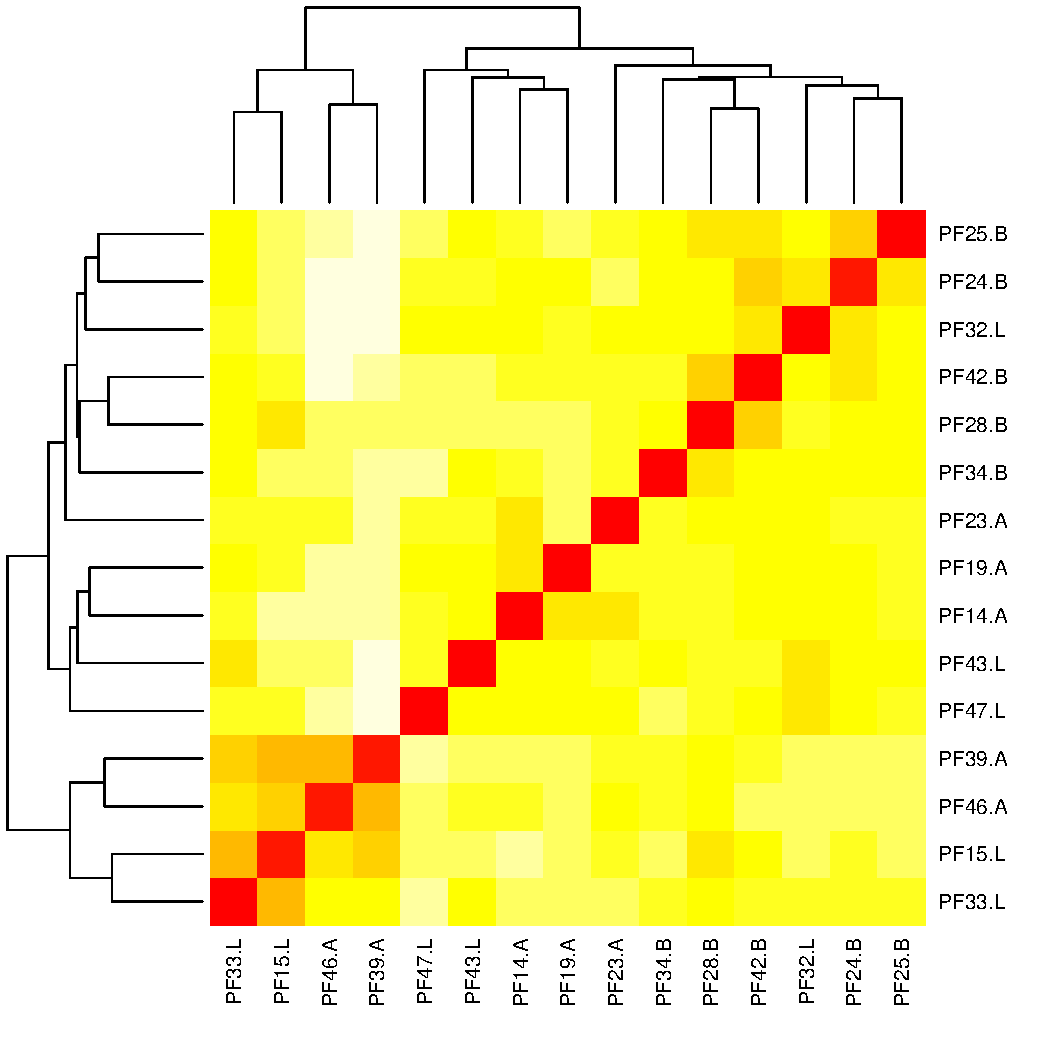
\includegraphics[width=\maxwidth]{images/graficdistAnalisis-1} 

\end{knitrout}
\caption{Mapa de colores de las distancias (euclídeas) entre los distintos arrays}
\label{fig:distArrays}
\end{figure}


Un cluster jerárquico seguido de un dendrograma nos puede ayudar a hacernos una idea de si las muestras se agrupan por condiciones experimentales. 

Si lo hacen es bueno, pero si no, no es necesariamente indicador de problemas, 
puesto que es un gráfico basado en todo los datos.

\begin{figure}
\centering
\begin{knitrout}
\definecolor{shadecolor}{rgb}{0.969, 0.969, 0.969}\color{fgcolor}
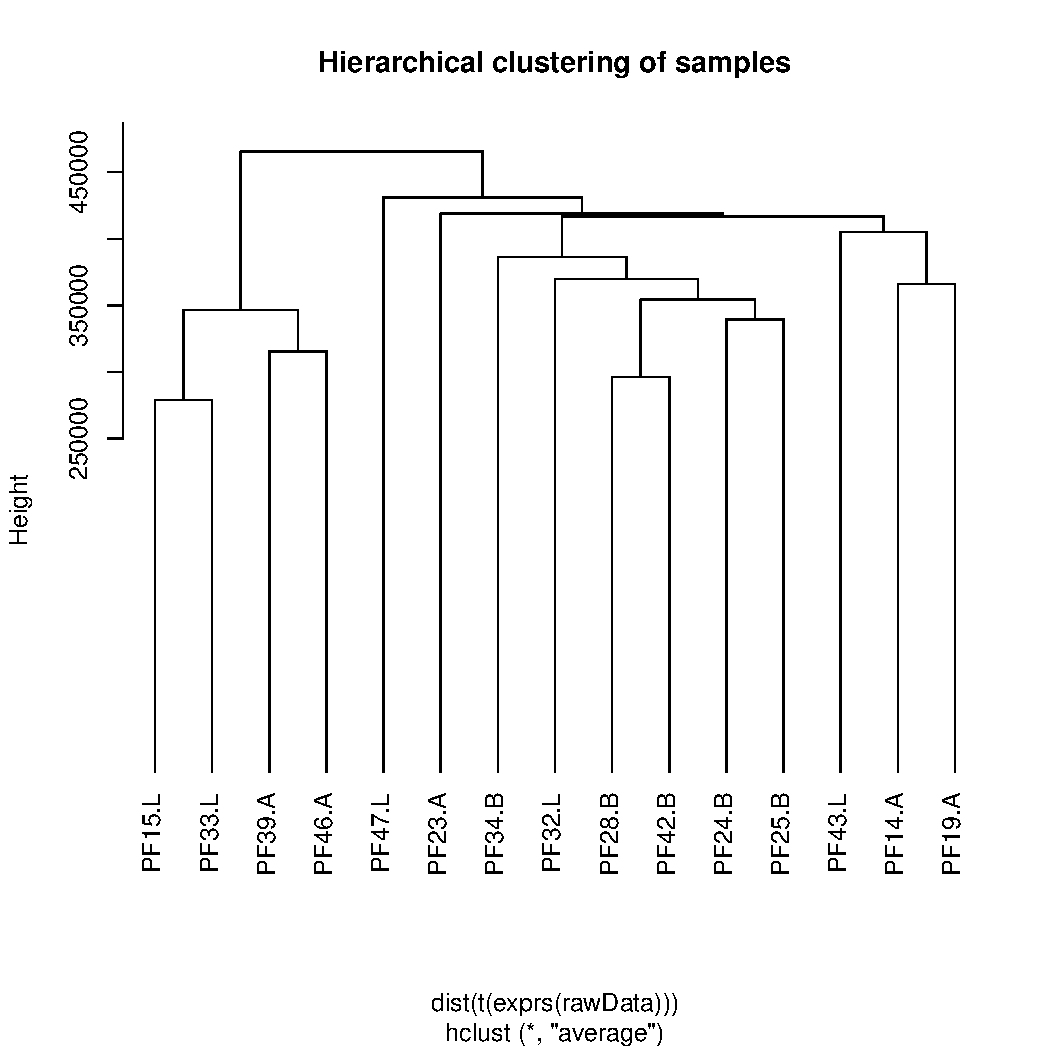
\includegraphics[width=\maxwidth]{images/graficplotDendro-1} 

\end{knitrout}
\caption{Dendrograma resultante de un agrupamiento jerárquico entre las muestras.
  Como en otras representaciones (Heatmaps, PCA) se observa una cierta agrupación de muestras de tipos similares aunque también una cierta heterogeneidad, atribuïble probablemente a la diferencia entre pacientes}
\label{fig:dendrograma}
\end{figure}

\subsubsection{Control de calidad (2): métodos específicos para microarrays}

El paquete \Rpackage{arrayQualitMetrics} encapsula todos los análisis anteriores, y alguno más, facilitando su ejecución e incluso su interpretación. La instrucción \texttt{arrayQualityMetrics} lleva a cabo todos los análisi de golpe y genera un informe de resultados con ayudas a la interpretación y a la detección de arrays problemáticos.

\begin{knitrout}
\definecolor{shadecolor}{rgb}{0.969, 0.969, 0.969}\color{fgcolor}\begin{kframe}
\begin{alltt}
\hlkwd{stopifnot}\hlstd{(}\hlkwd{require}\hlstd{(arrayQualityMetrics))}
\hlkwd{arrayQualityMetrics}\hlstd{(rawData,}
                    \hlkwc{intgroup} \hlstd{=} \hlstr{"Group"}\hlstd{,}
                    \hlkwc{outdir} \hlstd{=} \hlkwd{file.path}\hlstd{(resultsDir,} \hlstr{"arrayQuality"}\hlstd{),}
                    \hlkwc{force}\hlstd{=}\hlnum{TRUE}\hlstd{)}
\end{alltt}


{\ttfamily\noindent\itshape\color{messagecolor}{\#\# The report will be written into directory 'C:/Users/Alexandre/Dropbox (VHIR)/SotaCV/Ejemplo\_de\_MDA\_con\_Bioconductor/results/arrayQuality'.}}\end{kframe}
\end{knitrout}

\subsubsection{Archivos con los resultados del control de calidad}

Los resultados del control de calidad realizado con \texttt{arrayQualityMetrics} se encuentran  accesibles a traves del archivo \texttt{index.html} contenido en el subdirectorio creado al invocarlo -en este caso denominado \texttt{arrayQuality}.


\subsection{Normalizacion y Filtraje}

Una vez realizado el control de calidad se procede a normalizar los datos y sumarizarlos.

La normalización puede hacerse por distintos métodos (MAS5, VSN, RMA, GCRMA, ...) pero en este caso se utilizará el método RMA que es sin duda el más utilizado entre arrays de affymetrix.

El procesado mediante RMA implica un proceso en tres etapas: 
\begin{itemize}
\item Corrección de fondo (el RMA hace precisamente esto).
\item Normalización para hacer los valores de los arrays comparables.
\item Summarización de las diversas sondas asociadas a cada grupo de sondas para dar un único valor.
\end{itemize}


\begin{knitrout}
\definecolor{shadecolor}{rgb}{0.969, 0.969, 0.969}\color{fgcolor}\begin{kframe}
\begin{alltt}
\hlkwd{stopifnot}\hlstd{(}\hlkwd{require}\hlstd{(affy))}
\hlstd{eset_rma} \hlkwb{<-} \hlkwd{rma}\hlstd{(rawData)}
\end{alltt}
\begin{verbatim}
## Background correcting
## Normalizing
## Calculating Expression
\end{verbatim}
\end{kframe}
\end{knitrout}

Un boxplot de los valores normalizados muestra que los valores han quedado claramente en una escala común en donde se pueden comparar.
\begin{figure}[htbp]
\centering
\begin{knitrout}
\definecolor{shadecolor}{rgb}{0.969, 0.969, 0.969}\color{fgcolor}\begin{kframe}
\begin{alltt}
\hlkwd{boxplot}\hlstd{(eset_rma,}\hlkwc{main}\hlstd{=}\hlstr{"RMA"}\hlstd{,} \hlkwc{names}\hlstd{=sampleNames,} \hlkwc{cex.axis}\hlstd{=}\hlnum{0.7}\hlstd{,} \hlkwc{col}\hlstd{=colores,}\hlkwc{las}\hlstd{=}\hlnum{2}\hlstd{)}
\end{alltt}
\end{kframe}
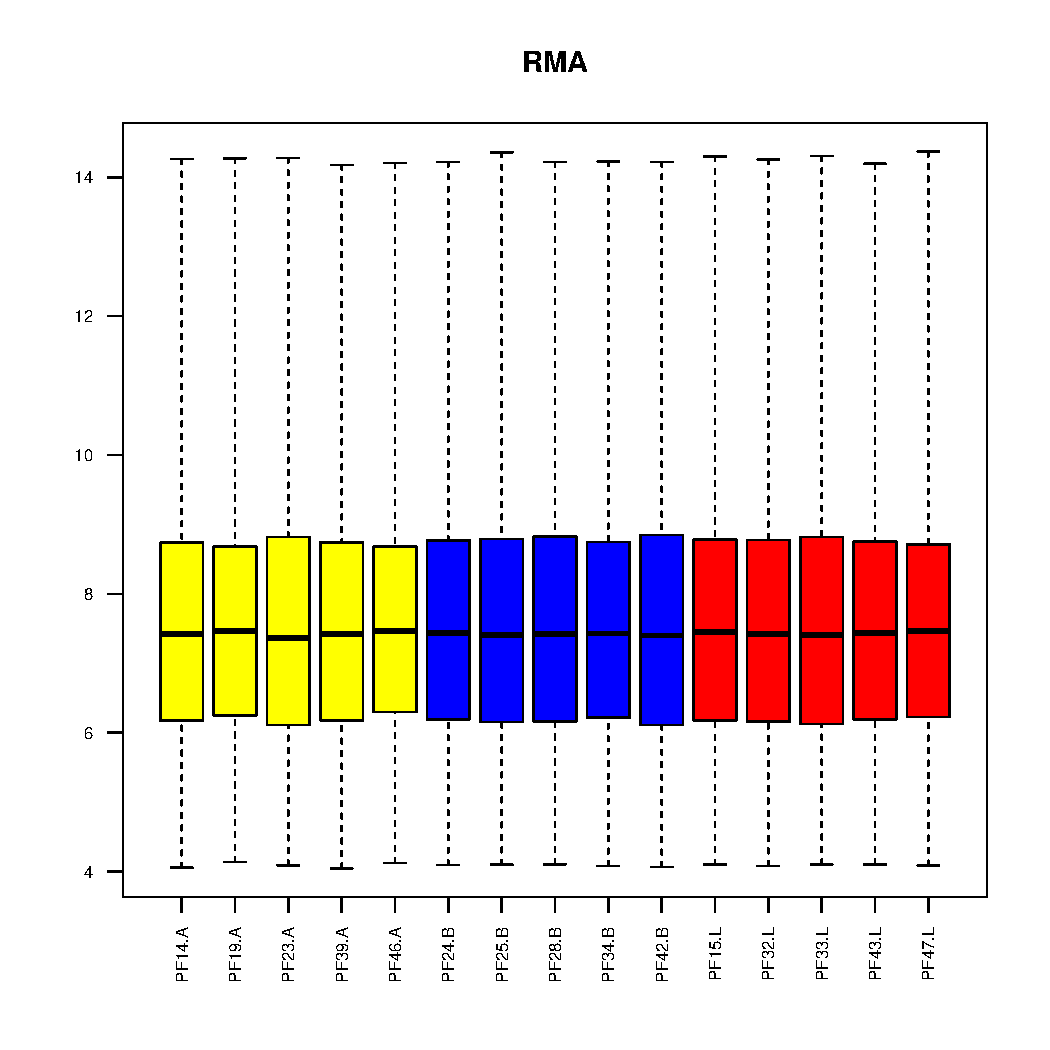
\includegraphics[width=\maxwidth]{images/graficnormBoxPlot-1} 

\end{knitrout}
\caption{El diagrama de cajas después de normalizar muestra como dicho proceso ha puesto los valores en una escala completamente comparable. \emph{Esto no significa que si hubieran errores los habría arreglado} por lo que dicho proceso debe hacerse tras descartar la ausencia de arrays problemáticos}
\label{fig:normboxplot}
\end{figure}

\subsubsection{Filtraje}

La selección de genes diferencialmente expresados se ve afectada por el número de genes sobre la que la hacemos. Cuántos más son, mayor será el ajuste necesario de p-valores (como se verá a continuación) lo que conllevará que podamos acabar descartando erróneamente más genes.

Por este motivo interesa reducir el total de genes que examinamos, es decir si podemos descartar los genes que, razonablemente no van a estar diferencialmente expresados podremos reducir el total sin apenas riesgo de descartar genes interesantes. Para ello podemos fijarnos, por ejemplo en la variabilidad global de cada gen, es decir sin tener en cuenta los grupos. La idea será que si un gen está diferencialmente expresado es preciso que haya una cierta diferencia entre los grupos, y por lo tanto la varianza global del gen será mayor que la de aquellos que no presentan expresión diferencial. Si hacemos un gráfico de la variabilidad de todos los genes, deberíamos poder diferenciar los genes que varian más (es decir que presentan expresión diferencial) de los que no la presentan. 

\begin{knitrout}
\definecolor{shadecolor}{rgb}{0.969, 0.969, 0.969}\color{fgcolor}\begin{kframe}
\begin{alltt}
\hlstd{sds} \hlkwb{<-} \hlkwd{apply} \hlstd{(}\hlkwd{exprs}\hlstd{(eset_rma),} \hlnum{1}\hlstd{, sd)}
\hlstd{sdsO}\hlkwb{<-} \hlkwd{sort}\hlstd{(sds)}
\hlkwd{plot}\hlstd{(}\hlnum{1}\hlopt{:}\hlkwd{length}\hlstd{(sdsO), sdsO,} \hlkwc{main}\hlstd{=}\hlstr{"Global variation over all genes"}\hlstd{)}
\end{alltt}
\end{kframe}
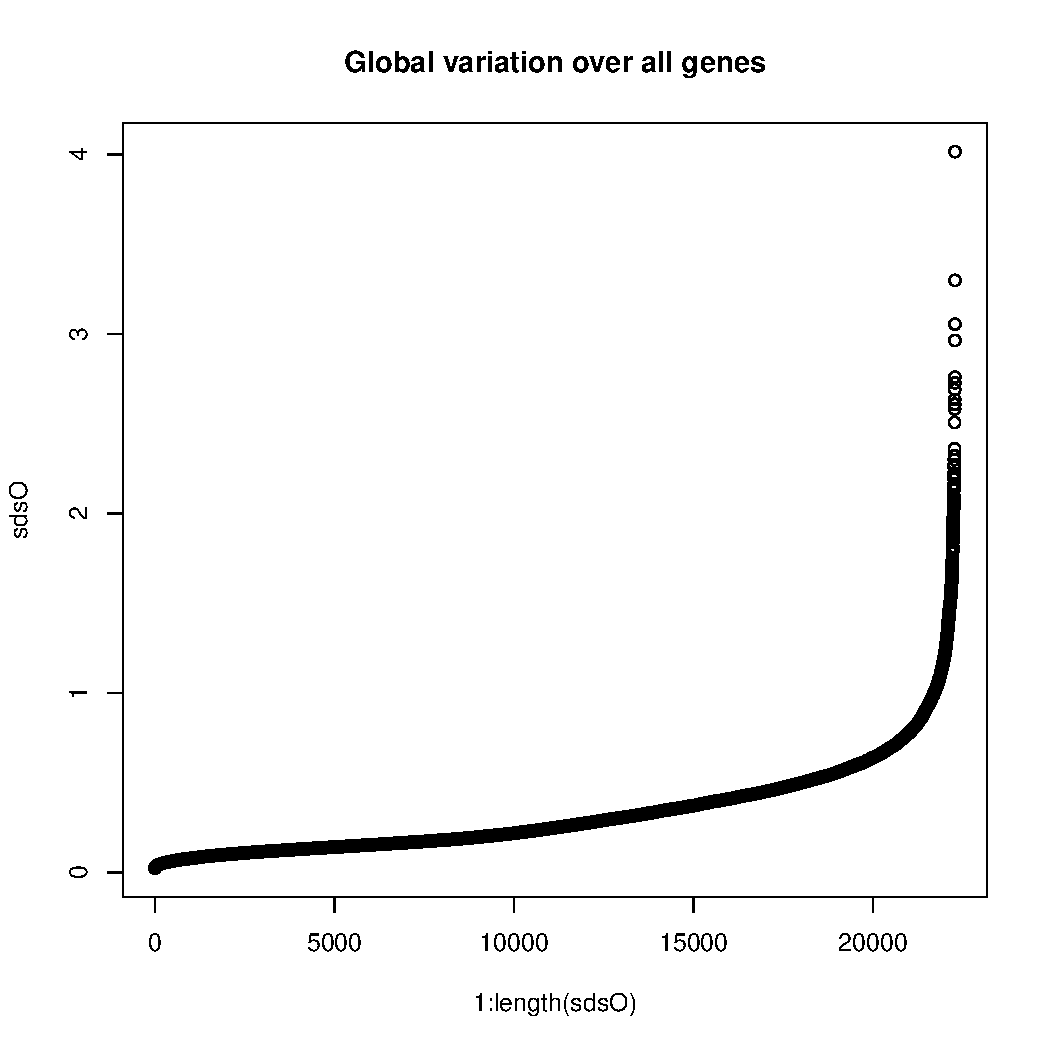
\includegraphics[width=\maxwidth]{images/graficvariancePlot-1} 

\end{knitrout}


El filtraje \emph{no específico} permite eliminar los genes que varían poco entre condiciones o que deseamos quitar por otras razones como por ejemplo que no disponemos de anotación para ellos. La función \texttt{nsFilter} permite eliminar los genes que, o bien varían poco, o bien no se dispone de anotación para ellos.

Si al filtrar deseamos usar las anotaciones, o la falta de ellas, como criterio de filtraje debemos disponer del correspondiente paquete de anotaciones.

\begin{knitrout}
\definecolor{shadecolor}{rgb}{0.969, 0.969, 0.969}\color{fgcolor}\begin{kframe}
\begin{alltt}
\hlkwd{require}\hlstd{(genefilter)}
\hlstd{filtered} \hlkwb{<-} \hlkwd{nsFilter}\hlstd{(eset_rma,} \hlkwc{require.entrez}\hlstd{=}\hlnum{TRUE}\hlstd{,}
         \hlkwc{remove.dupEntrez}\hlstd{=}\hlnum{TRUE}\hlstd{,} \hlkwc{var.func}\hlstd{=IQR,}
         \hlkwc{var.cutoff}\hlstd{=}\hlnum{0.5}\hlstd{,} \hlkwc{var.filter}\hlstd{=}\hlnum{TRUE}\hlstd{,}
         \hlkwc{filterByQuantile}\hlstd{=}\hlnum{TRUE}\hlstd{,} \hlkwc{feature.exclude}\hlstd{=}\hlstr{"^AFFX"}\hlstd{)}
\end{alltt}
\end{kframe}
\end{knitrout}

La función \texttt{nsFilter} devuelve los valores filtrados en un objeto \texttt{expressionSet} y un informe de los resultados del filtraje.

\begin{knitrout}
\definecolor{shadecolor}{rgb}{0.969, 0.969, 0.969}\color{fgcolor}\begin{kframe}
\begin{alltt}
\hlkwd{names}\hlstd{(filtered)}
\end{alltt}
\begin{verbatim}
## [1] "eset"       "filter.log"
\end{verbatim}
\begin{alltt}
\hlkwd{class}\hlstd{(filtered}\hlopt{$}\hlstd{eset)}
\end{alltt}
\begin{verbatim}
## [1] "ExpressionSet"
## attr(,"package")
## [1] "Biobase"
\end{verbatim}
\begin{alltt}
\hlkwd{print}\hlstd{(filtered}\hlopt{$}\hlstd{filter.log)}
\end{alltt}
\begin{verbatim}
## $numDupsRemoved
## [1] 7408
## 
## $numLowVar
## [1] 6219
## 
## $numRemoved.ENTREZID
## [1] 2428
## 
## $feature.exclude
## [1] 10
\end{verbatim}
\begin{alltt}
\hlstd{eset_filtered} \hlkwb{<-}\hlstd{filtered}\hlopt{$}\hlstd{eset}
\end{alltt}
\end{kframe}
\end{knitrout}

Podemos grabar el objeto \texttt{eset_rma} y los datos filtrados para su posterior uso.


\subsubsection{Archivos de resultados normalizados}

El resultado de la normalización y el filtraje es un objeto \texttt{expressionSet} almacenado en un archivo binario \texttt{datos.normaliados.Rda}, que será la base para todos los estudios posteriores.


Es muy común también que los investigadores deseen ver los datos normalizados por lo que también se pueden guardar en un archivo de texto para facilitar su posterior inspección. El archivo \texttt{Datos.Normalizados.Filtrados.csv2} contiene los datos normalizados y filtrados separados por ``;'' para no generar problemas de formato con el punto decimal en ingles o español.

\begin{knitrout}
\definecolor{shadecolor}{rgb}{0.969, 0.969, 0.969}\color{fgcolor}\begin{kframe}
\begin{alltt}
\hlstd{shortNames}\hlkwb{<-} \hlkwd{paste}\hlstd{(}\hlkwd{pData}\hlstd{(eset_rma)}\hlopt{$}\hlstd{Group,} \hlkwd{pData}\hlstd{(eset_rma)}\hlopt{$}\hlstd{SampleIDs,}\hlkwc{sep}\hlstd{=}\hlstr{"."}\hlstd{)}
\hlkwd{sum}\hlstd{(}\hlkwd{rownames}\hlstd{(}\hlkwd{pData}\hlstd{(eset_filtered))}\hlopt{!=}\hlkwd{colnames}\hlstd{(}\hlkwd{exprs}\hlstd{(eset_filtered)))}
\end{alltt}
\begin{verbatim}
## [1] 0
\end{verbatim}
\begin{alltt}
\hlkwd{colnames}\hlstd{(}\hlkwd{exprs}\hlstd{(eset_filtered))}\hlkwb{<-} \hlkwd{colnames}\hlstd{(}\hlkwd{exprs}\hlstd{(eset_rma))}\hlkwb{<-} \hlstd{shortNames}
\end{alltt}


{\ttfamily\noindent\bfseries\color{errorcolor}{\#\# Error in (function (od, vd) : object and replacement value dimnames differ}}\begin{alltt}
\hlkwd{write.csv2}\hlstd{(}\hlkwd{exprs}\hlstd{(eset_rma),} \hlkwd{file.path}\hlstd{(resultsDir,} \hlstr{"Datos.Normalizados.csv2"}\hlstd{))}
\hlkwd{write.csv2}\hlstd{(}\hlkwd{exprs}\hlstd{(eset_filtered),} \hlkwd{file.path}\hlstd{(resultsDir,} \hlstr{"Datos.Normalizados.Filtrados.csv2"}\hlstd{))}
\hlkwd{save}\hlstd{(eset_rma, eset_filtered,} \hlkwc{file}\hlstd{=}\hlkwd{file.path}\hlstd{(resultsDir,} \hlstr{"datos.normalizados.Rda"}\hlstd{))}
\end{alltt}
\end{kframe}
\end{knitrout}


\section{Selección de genes diferencialmente expresados}

Como en las etapas anteriores la selección de genes diferencialmente expresados (GDE) puede basarse en distintas aproximaciones, desde la $t$ de Student, tests de permutaciones o multitud de variantes.

Empezaremos realizando una comparación entre los grupos A y B que nos permitirá introducir algunos conceptos como el ajuste de p-valores para continuar luego con una aproximación más general, la utilización del modelo lineal que facilita la realización simultanea de más de dos comparaciones.

\subsection{Seleccion básica de genes en una comparación entre dos grupos}

Empezamos considerando el caso sencillo: Buscamos genes diferencialmente expresados entre dos condiciones utilizando un test clásico como el test$-t$.

\subsubsection{Cálculo de estadísticos de test y p--valores}

Una aproximación ``naïf'' a este análisis podría hacerse creando una función que calcule el test $t$ de Student y extraiga el p--valor y el valor de test. Aplicando esta función sobre toda la matiz de expresión y ordenando los valores resultantes de menor a mayor p--valor tendríamos una lista de candidatos a genes diferencialmente expresados.

Una versión algo mejorada de esta aproximación puede obtenerse aplicando la función \texttt{rowttests} del paquete
 \Rpack{genefilter} que calcula los estadísticos de test para cada fila de la matriz de expresión y devuelve, 
 para cada gen los valores del estadístico $t$, el $p$--valor, los grados de libertad  la diferencia de medias.
 
Escribiendo \texttt{? rowttests} se puede ver qué opciones hay disponibles.

La llamada a la función se hace pasándole el objeto y un campo tipo factor que diferencíe los dos grupos.

Crearemos un subconjunto de los datos tomando tan solo los grupos A y B.

\begin{knitrout}
\definecolor{shadecolor}{rgb}{0.969, 0.969, 0.969}\color{fgcolor}\begin{kframe}
\begin{alltt}
\hlstd{eset2} \hlkwb{<-} \hlstd{eset_filtered[,}\hlnum{1}\hlopt{:}\hlnum{10}\hlstd{]}
\hlkwd{pData}\hlstd{(eset2)}
\end{alltt}
\begin{verbatim}
##                Sample             Ids SampleIDs Group Apocrine.grade
## GSM26878.CEL GSM26878 PF14 EnPnT2N1G2      PF14     A              3
## GSM26883.CEL GSM26883 PF19 EnPuT4N0Gu      PF19     A              2
## GSM26887.CEL GSM26887 PF23 EnPnT2N0G2      PF23     A              3
## GSM26903.CEL GSM26903 PF39 EnPuT4N0Gu      PF39     A              3
## GSM26910.CEL GSM26910 PF46 EnPnT4N1G3      PF46     A              3
## GSM26888.CEL GSM26888 PF24 EnPnTiN0G3      PF24     B              2
## GSM26889.CEL GSM26889 PF25 EnPnT3N2G2      PF25     B              1
## GSM26892.CEL GSM26892 PF28 EnPnT2N1G3      PF28     B              2
## GSM26898.CEL GSM26898 PF34 EnPnT3N1G3      PF34     B              1
## GSM26906.CEL GSM26906 PF42 EnPnT2N2G3      PF42     B             na
##              AR.repeat.length
## GSM26878.CEL               18
## GSM26883.CEL               18
## GSM26887.CEL               18
## GSM26903.CEL               17
## GSM26910.CEL               19
## GSM26888.CEL               NA
## GSM26889.CEL               21
## GSM26892.CEL               22
## GSM26898.CEL               17
## GSM26906.CEL               16
\end{verbatim}
\begin{alltt}
\hlkwd{dim}\hlstd{(}\hlkwd{exprs}\hlstd{(eset2))}
\end{alltt}
\begin{verbatim}
## [1] 6218   10
\end{verbatim}
\end{kframe}
\end{knitrout}

Observemos que esta instrucción ha creado un subconjunto tanto de las covariables como de los datos!!!

\begin{knitrout}
\definecolor{shadecolor}{rgb}{0.969, 0.969, 0.969}\color{fgcolor}\begin{kframe}
\begin{alltt}
\hlkwd{stopifnot}\hlstd{(}\hlkwd{require}\hlstd{(genefilter))}
\hlstd{teststat} \hlkwb{<-}\hlkwd{rowttests}\hlstd{(eset2,} \hlstr{"Group"}\hlstd{)}
\hlkwd{head}\hlstd{(teststat)}
\end{alltt}
\begin{verbatim}
##              statistic         dm     p.value
## 216705_s_at -1.2091620 -0.2994326 0.261120186
## 212607_at   -4.3506604 -1.1042224 0.002443108
## 209028_s_at -1.7677938 -0.4968775 0.115072401
## 202382_s_at -3.4956834 -0.6426245 0.008130368
## 203256_at   -0.3900989 -0.1973068 0.706644376
## 209451_at   -2.2829535 -0.8503465 0.051831823
\end{verbatim}
\end{kframe}
\end{knitrout}

Ordenando los genes de menor a mayor p--valor tenemos una lista de genes \emph{candidatos} 
a ser considerados diferencialmente expresados.

\begin{knitrout}
\definecolor{shadecolor}{rgb}{0.969, 0.969, 0.969}\color{fgcolor}\begin{kframe}
\begin{alltt}
\hlstd{topDown}\hlkwb{<-}\hlkwd{order}\hlstd{(teststat}\hlopt{$}\hlstd{p.value)}
\hlstd{ranked}\hlkwb{<-}\hlstd{teststat[topDown,]}
\hlkwd{print}\hlstd{(top10}\hlkwb{<-}\hlstd{ranked[}\hlnum{1}\hlopt{:}\hlnum{10}\hlstd{,])}
\end{alltt}
\begin{verbatim}
##             statistic        dm      p.value
## 214451_at    25.81132  5.665059 5.445929e-09
## 204667_at    25.08796  3.038344 6.819410e-09
## 214079_at    15.42509  6.032815 3.102260e-07
## 206509_at    14.84966  5.581047 4.166328e-07
## 218211_s_at  12.92792  2.682284 1.212997e-06
## 205044_at   -11.54100 -5.626206 2.884239e-06
## 208763_s_at  11.40712  1.184755 3.151220e-06
## 209786_at   -10.63889 -2.308988 5.335935e-06
## 215729_s_at -10.63444 -3.452290 5.352779e-06
## 202329_at   -10.39560 -0.602802 6.348918e-06
\end{verbatim}
\end{kframe}
\end{knitrout}

\paragraph{Volcano plots}

Un gráfico muy útil para hacerse una idea de si hay muchos o pocos genes cambiados es el \emph{volcano plot} que representa la significación de cada gen, medida por \emph{``menos el logaritmo del p--valor''} frente al cambio de expresión medido por el \texttt{fold--change} o diferencia de medias, que puede considerarse equivalente a una expresión relativa siempre que los datos se encuentren en una escala logarítmica (``el logaritmo del cociente es la diferencia de logaritmos'').

\begin{knitrout}
\definecolor{shadecolor}{rgb}{0.969, 0.969, 0.969}\color{fgcolor}\begin{kframe}
\begin{alltt}
\hlstd{x}\hlkwb{<-}\hlstd{ranked}\hlopt{$}\hlstd{dm; y}\hlkwb{<-}\hlopt{-}\hlkwd{log}\hlstd{(ranked}\hlopt{$}\hlstd{p.value)}
\hlkwd{plot}\hlstd{(x, y,} \hlkwc{xlab}\hlstd{=}\hlstr{"Fold Change"}\hlstd{,} \hlkwc{ylab} \hlstd{=}\hlstr{"-logPval"}\hlstd{,}
     \hlkwc{main}\hlstd{=}\hlstr{"Volcano plot\textbackslash{}nA vs B"}\hlstd{)}
\hlkwd{abline}\hlstd{(}\hlkwc{v}\hlstd{=}\hlopt{-}\hlnum{1}\hlstd{);}\hlkwd{abline}\hlstd{(}\hlkwc{v}\hlstd{=}\hlnum{1}\hlstd{);}
\hlkwd{text} \hlstd{(x[}\hlnum{1}\hlopt{:}\hlnum{10}\hlstd{], y[}\hlnum{1}\hlopt{:}\hlnum{10}\hlstd{],}\hlkwd{rownames}\hlstd{(ranked)[}\hlnum{1}\hlopt{:}\hlnum{10}\hlstd{],} \hlkwc{cex}\hlstd{=}\hlnum{0.7}\hlstd{)}
\end{alltt}
\end{kframe}
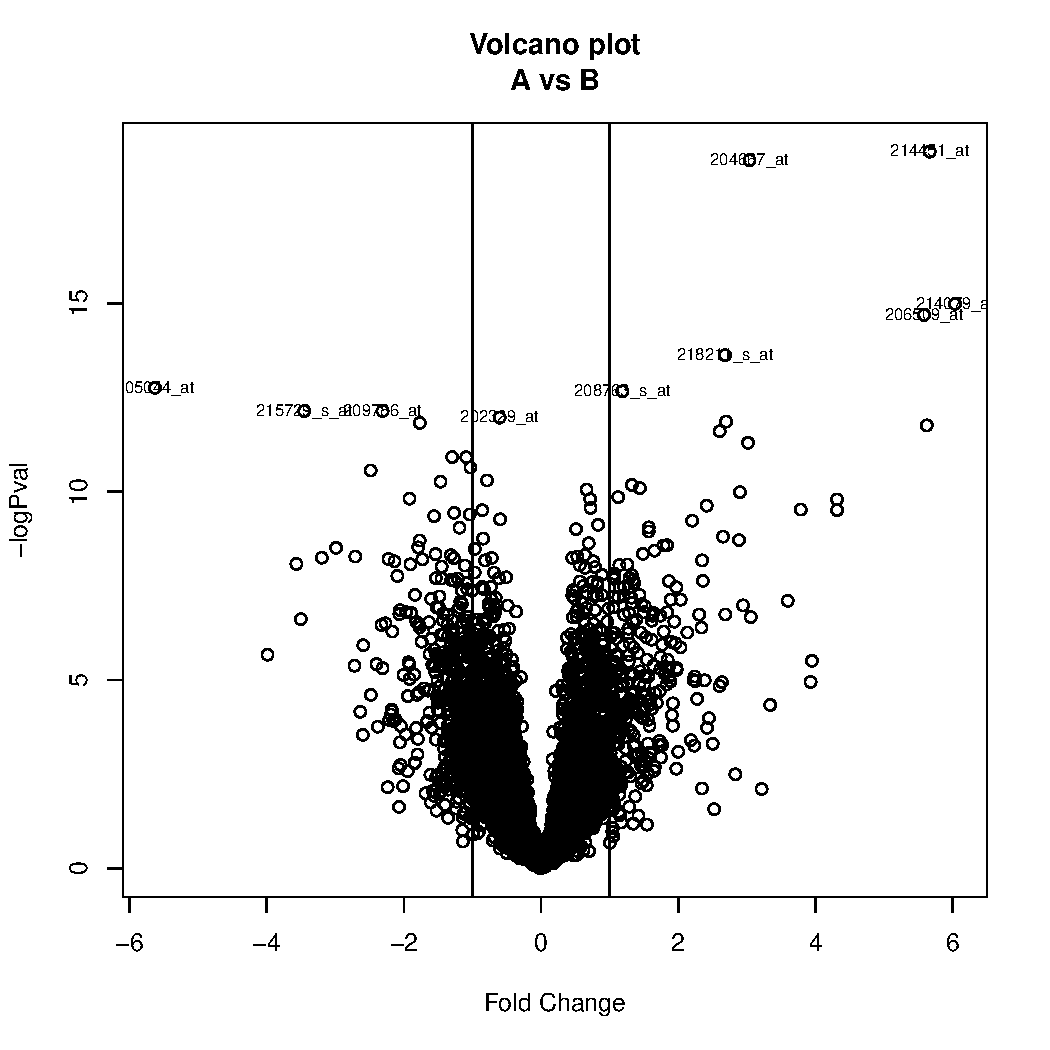
\includegraphics[width=\maxwidth]{images/graficvolcano1-1} 

\end{knitrout}

%\paragraph{Las variancias muy pequeñas pueden generar falsos positivos}
%Obsérvese que algunos genes tienen valores grandes de $t$ (pequeños de $p$) pero 
%una diferencia de medias baja, lo que sugiere que su varianza pueda ser muy pequeña y el p--valor se encuentre inflado artificialmente.
%Podemos calcular las desviaciones estándar y concatenarlas con el objeto anterior 
%lo que nos permitirá hacernos una idea de si ésto es así.

%<<addvariance>>=
%sds <- apply(exprs(eset2),1, sd)
%rankedSD <- sds[topDown]
%rankedWithSDs <- cbind(ranked, rankedSD)
%print(top25<-rankedWithSDs[1:10,])
%topDownSds <- order(rankedWithSDs$rankedSD)
%print(top25SD<-head(rankedWithSDs[topDownSds,], n=25))
%@ 

\paragraph{Alternativas al test $t$ de Student}

La utilización del test-$t$ se basa en la suposición de normalidad de los datos que deberíamos verificar, lo cual resulta difícil porque, gen a gen, se dispone sólo de 10 puntos.

A falta de dicha comprobación podríamos usar aproximaciones menos restrictivas como tests de permutaciones similares a los incluïdos en el paquete \texttt{multtest}. 

En este ejemplo y con fines ilustrativos aceptaremos que los p--valores obtenidos nos permite realizar una ordenación válida de los genes de más a menos diferencialmentee expresados.

Aún así subsisten varios problemas que deberíamos considerar:

\begin{itemize}
\item ¿Cómo podemos seleccionar los genes que deseamos considerar ``expresados diferencialmente''?
\item ¿Cómo podemos establecer una línea de corte que garantice un control similar ded error tipo I
al de los análisis estadísticos tradicionales?
\item ¿Como podemos, por lo menos,  obtener estimaciones decente de los porcentajes de falsos positivos y falsos negativos?
\end {itemize}

\subsubsection{Selección de los genes [más] expresados diferencialmente}

Suponiendo que consideramos válidas las condiciones para aplicar el test--t podemos clasificar los genes por sus p--valores y seleccionar algunos de los genes de la parte superior de la lista (es decir los que tienen menor p-valor)

\begin{knitrout}
\definecolor{shadecolor}{rgb}{0.969, 0.969, 0.969}\color{fgcolor}\begin{kframe}
\begin{alltt}
\hlstd{selectedNaif} \hlkwb{<-}\hlstd{ranked[ranked}\hlopt{$}\hlstd{p.value}\hlopt{<}\hlnum{0.01}\hlstd{,]}
\hlkwd{nrow}\hlstd{(selectedNaif)}
\end{alltt}
\begin{verbatim}
## [1] 650
\end{verbatim}
\end{kframe}
\end{knitrout}

Sin embargo, el hecho de que estamos haciendo miles de pruebas al mismo tiempo puede inducir a error.
Una posibilidad es ajustar los p--valores de tal manera que se obtenga algún tipo
de \emph{control de la tasa de error global}, es decir la probabilidad de obtener falsos positivos, no con una sino con todas las comparaciones.

Otra posibilidad es estimar la \emph{tasa de falsos positivos o ``False Discovery Rate'' (FDR)}, el porcentaje de falsos positivos entre los genes considerados positivos.

En este caso nos centraremos en la primera opción, ajustar los p--valores.

\subsubsection{Ajuste de p--valores para comparaciones múltiples}

El ajuste para pruebas múltiples de los p--valores permite obtener un control global
de la probabilidad de considerar equivocadamente un gen como diferencialmente expresado.

Es decir, si seleccionamos los genes cuyos p--valores ajustados, $p^*$ están por debajo de un umbral determinado, ($p^* \leq \alpha$), significa que en lugar de hacer
las pruebas con un error tipo I de $\alpha$  las hacemos con una FDR (o FWER) esperada
igual o inferior a $\alpha $.

Hay muchos métodos para ajustar los p--valores. El paquete \Rpack{multtest} proporciona funciones sencillas que permiten realizar los ajustes más usuales.

\begin{knitrout}
\definecolor{shadecolor}{rgb}{0.969, 0.969, 0.969}\color{fgcolor}\begin{kframe}
\begin{alltt}
\hlkwd{stopifnot}\hlstd{(}\hlkwd{require}\hlstd{(multtest))}
\hlcom{#procs <- c("Bonferroni","Holm","Hochberg","SidakSS","SidakSD","BH", "BY")}
\hlstd{procs} \hlkwb{<-} \hlkwd{c}\hlstd{(}\hlstr{"Bonferroni"}\hlstd{,}\hlstr{"BH"}\hlstd{)}
\hlstd{adjPvalues} \hlkwb{<-} \hlkwd{mt.rawp2adjp}\hlstd{(ranked}\hlopt{$}\hlstd{p.value, procs)}
\hlkwd{names}\hlstd{(adjPvalues)}
\end{alltt}
\begin{verbatim}
## [1] "adjp"    "index"   "h0.ABH"  "h0.TSBH"
\end{verbatim}
\begin{alltt}
\hlstd{ranked.adjusted}\hlkwb{<-}\hlkwd{cbind}\hlstd{(ranked[,}\hlkwd{c}\hlstd{(}\hlnum{1}\hlstd{,}\hlnum{3}\hlstd{)], adjPvalues}\hlopt{$}\hlstd{adjp[,}\hlopt{-}\hlnum{1}\hlstd{])}
\hlstd{ranked.adjusted[}\hlnum{1}\hlopt{:}\hlnum{10}\hlstd{,]}
\end{alltt}
\begin{verbatim}
##             statistic      p.value   Bonferroni           BH
## 214451_at    25.81132 5.445929e-09 3.386279e-05 2.120155e-05
## 204667_at    25.08796 6.819410e-09 4.240309e-05 2.120155e-05
## 214079_at    15.42509 3.102260e-07 1.928985e-03 6.429951e-04
## 206509_at    14.84966 4.166328e-07 2.590623e-03 6.476558e-04
## 218211_s_at  12.92792 1.212997e-06 7.542414e-03 1.508483e-03
## 205044_at   -11.54100 2.884239e-06 1.793420e-02 2.799184e-03
## 208763_s_at  11.40712 3.151220e-06 1.959428e-02 2.799184e-03
## 209786_at   -10.63889 5.335935e-06 3.317884e-02 3.698176e-03
## 215729_s_at -10.63444 5.352779e-06 3.328358e-02 3.698176e-03
## 202329_at   -10.39560 6.348918e-06 3.947757e-02 3.731624e-03
\end{verbatim}
\end{kframe}
\end{knitrout}

Como puede verse el número de genes seleccionado si fijáramos el mismo punto de corte sería inferior a si no lo hiciéramos Con los p--valores ajustados podemos usar puntos de corte de 0.01 o 0.05 y, si el ajuste controla la tasa de falsos positivos, este valor puede subir hasta 0.25 puesto que lo que indicaría es que si declaráramos diferencialmente expresados los genes con un p--valor ajustado menor o igual que aquel esperaríamos que, de cada 100 que verificáramos se encontraran 25 falsos positivos, lo que puede resultar perfectamente aceptable en estudios exploratorios.

\begin{knitrout}
\definecolor{shadecolor}{rgb}{0.969, 0.969, 0.969}\color{fgcolor}\begin{kframe}
\begin{alltt}
\hlstd{selectedAdjusted}\hlkwb{<-}\hlstd{ranked.adjusted[ranked.adjusted}\hlopt{$}\hlstd{BH}\hlopt{<}\hlnum{0.01}\hlstd{,]}
\hlkwd{nrow}\hlstd{(selectedAdjusted)}
\end{alltt}
\begin{verbatim}
## [1] 19
\end{verbatim}
\begin{alltt}
\hlstd{selectedAdjusted2}\hlkwb{<-}\hlstd{ranked.adjusted[ranked.adjusted}\hlopt{$}\hlstd{BH}\hlopt{<}\hlnum{0.05}\hlstd{,]}
\hlkwd{nrow}\hlstd{(selectedAdjusted2)}
\end{alltt}
\begin{verbatim}
## [1] 228
\end{verbatim}
\begin{alltt}
\hlstd{selectedAdjusted2}\hlkwb{<-}\hlstd{ranked.adjusted[ranked.adjusted}\hlopt{$}\hlstd{BH}\hlopt{<}\hlnum{0.25}\hlstd{,]}
\hlkwd{nrow}\hlstd{(selectedAdjusted2)}
\end{alltt}
\begin{verbatim}
## [1] 1888
\end{verbatim}
\end{kframe}
\end{knitrout}


\subsection{Análisis basado en modelos lineales}

Como se ha indicado en la introducción a este apartado, cuando hay más de dos grupos la aproximación natural es realizar algun tipo de análisis de la varianza.

En este ejemplo, se aplicará la aproximación desarrollada por Smyth \emph{et al.} (2004) basado en la utilización del \emph{modelo lineal general} combinada con un método 
para obtener una estimación mejorada de la varianza. Dicho método se conoce con el mismo nombre del paquete: \texttt{limma} por \emph{linear models for microarray data}.


\subsubsection{Matrices de diseño y de contrastes}

El primer paso para el análisis basado en modelos lineales es crear la matriz de diseño.
Básicamente se trata de una tabla que describe la asignación de cada muestra a un grupo. Tiene tantas filas como muestras y tantas columnas como grupos (si solo se considera un factor)Cada fila contiene un uno en la columna del grupo al que pertenece la muestra y un cero en las restantes.

La matriz de contrastes esse utiliza para describir las comparaciones entre grupos. Consta de tantas columnas como comparaciones y tantas filas como grupos (es decir como columnas de la matriz de diseño). Una comparaci\'on entre grupos --lamada ``contraste''-- se representa con un ``1'' y un ``-1'' en las filas de los grupos a comparar y ceros en las restantes. Si varios grupos intervinieran en la comparaci\'on se tendría tantos coeeficientes como grupos con la única restricción de que su suma sería cero. 

La matriz de diseño puede definirse manualmente o a partir de un factor 
creado específicamente para ello.

Manualmente, seria:
\begin{knitrout}
\definecolor{shadecolor}{rgb}{0.969, 0.969, 0.969}\color{fgcolor}\begin{kframe}
\begin{alltt}
\hlstd{design}\hlkwb{<-}\hlkwd{matrix}\hlstd{(}
            \hlkwd{c}\hlstd{(}\hlnum{1}\hlstd{,}\hlnum{1}\hlstd{,}\hlnum{1}\hlstd{,}\hlnum{1}\hlstd{,}\hlnum{1}\hlstd{,}\hlnum{0}\hlstd{,}\hlnum{0}\hlstd{,}\hlnum{0}\hlstd{,}\hlnum{0}\hlstd{,}\hlnum{0}\hlstd{,}\hlnum{0}\hlstd{,}\hlnum{0}\hlstd{,}\hlnum{0}\hlstd{,}\hlnum{0}\hlstd{,}\hlnum{0}\hlstd{,}
              \hlnum{0}\hlstd{,}\hlnum{0}\hlstd{,}\hlnum{0}\hlstd{,}\hlnum{0}\hlstd{,}\hlnum{0}\hlstd{,}\hlnum{1}\hlstd{,}\hlnum{1}\hlstd{,}\hlnum{1}\hlstd{,}\hlnum{1}\hlstd{,}\hlnum{1}\hlstd{,}\hlnum{0}\hlstd{,}\hlnum{0}\hlstd{,}\hlnum{0}\hlstd{,}\hlnum{0}\hlstd{,}\hlnum{0}\hlstd{,}
              \hlnum{0}\hlstd{,}\hlnum{0}\hlstd{,}\hlnum{0}\hlstd{,}\hlnum{0}\hlstd{,}\hlnum{0}\hlstd{,}\hlnum{0}\hlstd{,}\hlnum{0}\hlstd{,}\hlnum{0}\hlstd{,}\hlnum{0}\hlstd{,}\hlnum{0}\hlstd{,}\hlnum{1}\hlstd{,}\hlnum{1}\hlstd{,}\hlnum{1}\hlstd{,}\hlnum{1}\hlstd{,}\hlnum{1}\hlstd{),}
            \hlkwc{nrow}\hlstd{=}\hlnum{15}\hlstd{,}\hlkwc{byrow}\hlstd{=F)}
\hlkwd{colnames}\hlstd{(design)}\hlkwb{<-}\hlkwd{c}\hlstd{(}\hlstr{"A"}\hlstd{,} \hlstr{"B"}\hlstd{,} \hlstr{"L"}\hlstd{)}
\hlkwd{rownames}\hlstd{(design)} \hlkwb{<-}  \hlstd{sampleNames}
\hlkwd{print}\hlstd{(design)}
\end{alltt}
\begin{verbatim}
##        A B L
## PF14.A 1 0 0
## PF19.A 1 0 0
## PF23.A 1 0 0
## PF39.A 1 0 0
## PF46.A 1 0 0
## PF24.B 0 1 0
## PF25.B 0 1 0
## PF28.B 0 1 0
## PF34.B 0 1 0
## PF42.B 0 1 0
## PF15.L 0 0 1
## PF32.L 0 0 1
## PF33.L 0 0 1
## PF43.L 0 0 1
## PF47.L 0 0 1
\end{verbatim}
\end{kframe}
\end{knitrout}

Las comparaciones que nos interesan son las diferencias, dos a dos entre cada tipo de tumor lo que puede hacerse con los contrastes siguientes:

\begin{knitrout}
\definecolor{shadecolor}{rgb}{0.969, 0.969, 0.969}\color{fgcolor}\begin{kframe}
\begin{alltt}
\hlkwd{require}\hlstd{(limma)}
\hlstd{cont.matrix} \hlkwb{<-} \hlkwd{makeContrasts} \hlstd{(}
      \hlkwc{AvsB} \hlstd{= B}\hlopt{-}\hlstd{A,}
      \hlkwc{AvsL} \hlstd{= L}\hlopt{-}\hlstd{A,}
      \hlkwc{BvsL} \hlstd{= L}\hlopt{-}\hlstd{B,}
      \hlkwc{levels}\hlstd{=design)}
\hlkwd{print}\hlstd{(cont.matrix)}
\end{alltt}
\begin{verbatim}
##       Contrasts
## Levels AvsB AvsL BvsL
##      A   -1   -1    0
##      B    1    0   -1
##      L    0    1    1
\end{verbatim}
\end{kframe}
\end{knitrout}

\subsubsection{Estimación del modelo y selección de genes}

Una vez definida la matriz de diseño y los contrastes podemos pasar a estimar 
el modelo, estimar los contrastes y realizar las pruebas de significación 
que nos indiquen, para cada gen y cada comparaci\'on, 
si puede considerarse diferencialmente expresado.



El método implementado en \Rpackage {limma} amplía el análisis tradicional 
utilizando modelos de Bayes empíricos para combinar la información de toda la matriz de datos y de cada gen individual y  obtener estimaciones de error mejoradas.

El análisis proporciona los estadísticos de test habituales como \texttt{Fold--change}
$t$-moderados o $p$-valores ajustados que se utilizan para ordenar los genes de mas a menos diferencialmente expresados.

A fin de controlar el porcentaje de falsos positivos que puedan resultar del alto numero de contrastes realizados simultaneamente
los p--valores se ajustan de forma que tengamos control sobre la tasa de falsos positivos utilizando el metodo 
de Benjamini y Hochberg (\cite{BenjaminiHochberg:1995}). 

La funcion \texttt{topTable} genera para cada contraste una lista de genes 
ordenados de mas a menos diferencialmente expresados.

\begin{knitrout}
\definecolor{shadecolor}{rgb}{0.969, 0.969, 0.969}\color{fgcolor}\begin{kframe}
\begin{alltt}
\hlstd{topTab_AvsB} \hlkwb{<-} \hlkwd{topTable} \hlstd{(fit.main,} \hlkwc{number}\hlstd{=}\hlkwd{nrow}\hlstd{(fit.main),} \hlkwc{coef}\hlstd{=}\hlstr{"AvsB"}\hlstd{,} \hlkwc{adjust}\hlstd{=}\hlstr{"fdr"}\hlstd{)}
\hlstd{topTab_AvsL} \hlkwb{<-} \hlkwd{topTable} \hlstd{(fit.main,} \hlkwc{number}\hlstd{=}\hlkwd{nrow}\hlstd{(fit.main),} \hlkwc{coef}\hlstd{=}\hlstr{"AvsL"}\hlstd{,} \hlkwc{adjust}\hlstd{=}\hlstr{"fdr"}\hlstd{)}
\hlstd{topTab_BvsL}  \hlkwb{<-} \hlkwd{topTable} \hlstd{(fit.main,} \hlkwc{number}\hlstd{=}\hlkwd{nrow}\hlstd{(fit.main) ,} \hlkwc{coef}\hlstd{=}\hlstr{"BvsL"}\hlstd{,} \hlkwc{adjust}\hlstd{=}\hlstr{"fdr"}\hlstd{)}
\end{alltt}
\end{kframe}
\end{knitrout}

Los volcano-plots permiten visualizar si hay muchos o pocos genes con un gran fold-change y significativamente expresados o si este número es bajo. Estos gráficos representa en abscisas los cambios de expresión en escala logarítmica
y en ordenadas el ``menos logaritmo'' del p-valor o alternativamente el estadístico $B$ (``log-odds'').




\subsubsection{Principales genes expresados diferencialmente}

Si consideráramos genes expresados diferencialmente aquellos que tienen un p--valor ajustado inferior a $0.05$ o $0.01$ el número de genes diferencialmente expresado en cada caso sería:




Los 10 genes más expresados diferencialmente en cada comparaci\'on se muestran en las tablas siguientes:








\section{Post-procesado de las listas de genes obtenidas}

Una vez obtenidas las listas de genes diferencialmente expresados pueden llevarse a cabo todo tipo de análisis sobre ellas, generalmente encaminados a facilitar la interpretación de los resultados.

Entre estas exploraciones --que podemos llamar genericamente ``post-procesado de las listas'' se encuentra

\begin{itemize}
\item La anotación de las listas de genes en diversas bases de datos.

\item La comparaci\'on entre las listas para determinar que genes cambian simultaneamente -o no- en varias comparaciones (o cuales cambian en una comparaci\'on pero no en otra).
\item La visualización de todos los genes seleccionados en varias comparaciones para, de forma similar a lo anterior, detectar grupos de genes con patrones de cambio similares --o distintos-- entre distintas comparaciones.
\item EL análisis de significación biológica de las listas mediante análisis de enriquecimiento o mediante ``gene set analysis'' para detectar si las listas se encuentran enriquecidas en genes asociados a funciones o procesos biológicos determinados.
\end{itemize}


\subsection{Comparaciones múltiples}

Cuando se realizan varias comparaciones a la vez puede resultar importante ver 
que genes cambian simultáneamente en más de una comparaci\'on.
Si el número de comparaciones es alto también puede ser necesario realizar un 
ajuste de p-valores entre las comparaciones, distinto del realizado entre genes.

La función \texttt{decidetests} permite realizar ambas cosas.
En este ejemplo no se ajustaran los p--valores entre comparaciones. Tan solo se seleccionaran los genes que cambian en una o más condiciones.

EL resultado del análisis es una tabla \texttt{res} que para cada gen y cada comparaci\'on 
contiene un 1 (si el gen esta sobre-expresado o ``up'' en esta condicion), 
un 0 (si no hay cambio significativo) o un -1 
(si esta ``down''-regulado).



Para resumir dicho análisis podemos contar qué filas tienen como mínimo una celda distinta de cero:

\begin{knitrout}
\definecolor{shadecolor}{rgb}{0.969, 0.969, 0.969}\color{fgcolor}\begin{kframe}
\begin{alltt}
\hlstd{sum.res.rows}\hlkwb{<-}\hlkwd{apply}\hlstd{(}\hlkwd{abs}\hlstd{(res),}\hlnum{1}\hlstd{,sum)}
\hlstd{res.selected}\hlkwb{<-}\hlstd{res[sum.res.rows}\hlopt{!=}\hlnum{0}\hlstd{,]}
\hlkwd{print}\hlstd{(}\hlkwd{summary}\hlstd{(res))}
\end{alltt}
\begin{verbatim}
##    AvsB AvsL BvsL
## -1   88   11   19
## 0  6037 6193 6175
## 1    93   14   24
\end{verbatim}
\end{kframe}
\end{knitrout}

En vista de estos valores podemos aplicar otros criterios de selección, por ejemplo genes con un p-valor ajustado inferior a 0.05 y \texttt{log Fold change} mayor o igual a 1.\emph{ Este criterio combina a la vez la significación estadística y la significación biológica por lo que, en un estudio real sería probablemente el escogido}.

\begin{knitrout}
\definecolor{shadecolor}{rgb}{0.969, 0.969, 0.969}\color{fgcolor}\begin{kframe}
\begin{verbatim}
##    AvsB AvsL BvsL
## -1  191   36   55
## 0  5784 6138 6086
## 1   243   44   77
\end{verbatim}
\end{kframe}
\end{knitrout}

Un diagrama de Venn permite visualizar la tabla anterior sin diferenciar entre genes ``up'' o ``down'' regulados.

\begin{figure}
\begin{knitrout}
\definecolor{shadecolor}{rgb}{0.969, 0.969, 0.969}\color{fgcolor}\begin{kframe}
\begin{alltt}
\hlkwd{vennDiagram} \hlstd{(res.selected[,}\hlnum{1}\hlopt{:}\hlnum{3}\hlstd{],} \hlkwc{main}\hlstd{=}\hlstr{"Genes in common #1"}\hlstd{,} \hlkwc{cex}\hlstd{=}\hlnum{0.9}\hlstd{)}
\end{alltt}
\end{kframe}
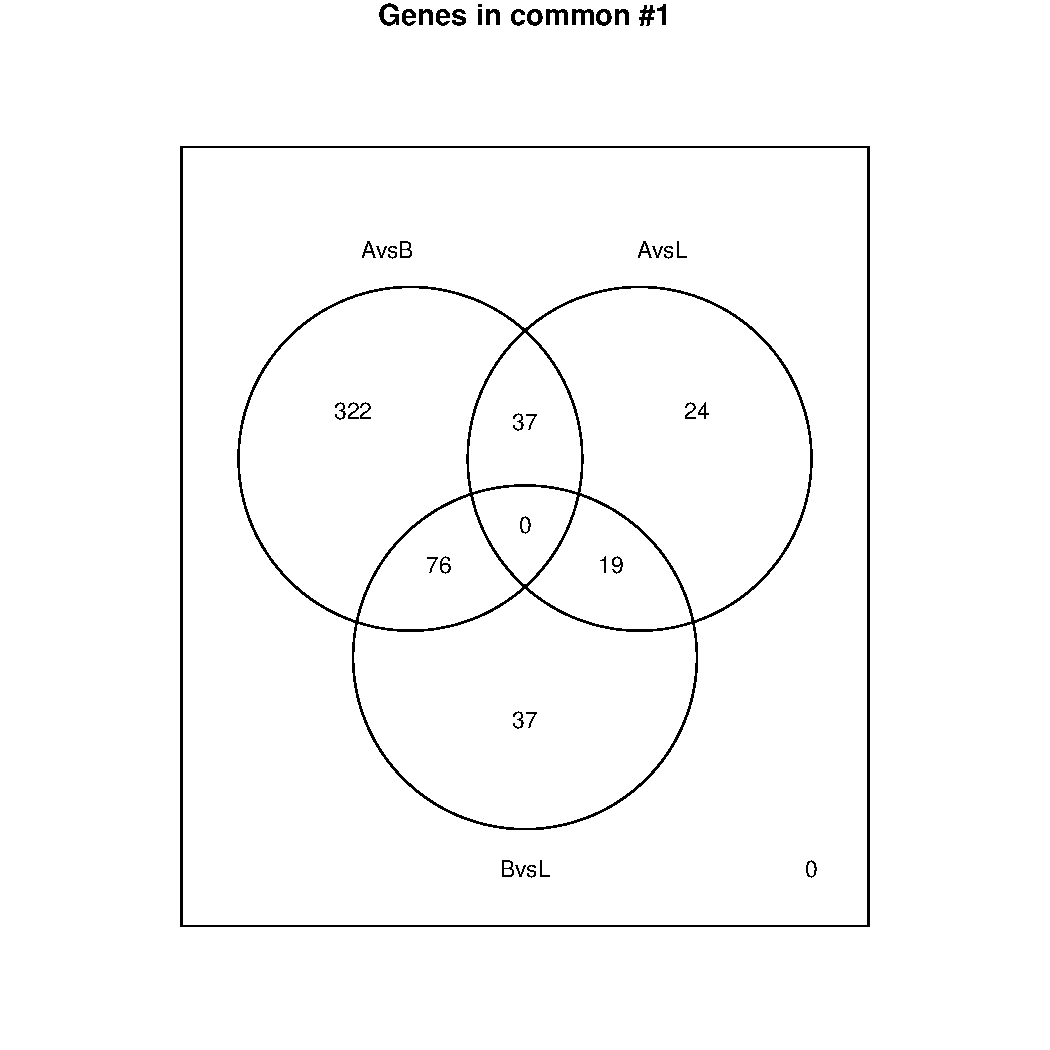
\includegraphics[width=\maxwidth]{images/graficvenn1-1} 

\end{knitrout}
\caption{\label{venn1}Número de genes seleccionado en cada comparaci\'on}
\end{figure}


\subsection{Anotación de resultados}

La identificación de los genes seleccionados puede resultar más sencilla para el especialista en un campo si se utilizan nombres estándar como el simbolo del gen o ``gene symbol''.
Con esta finalidad cada paquete de anotaciones tiene tablas de correspondencia entre los distintos tipos de identificadores, principalmente entre los del array y los de otras bases de datos.

Para saber que anotaciones estan disponibles debe cargarse el paquete y llamar la función del mismo nombre 

\begin{knitrout}
\definecolor{shadecolor}{rgb}{0.969, 0.969, 0.969}\color{fgcolor}\begin{kframe}
\begin{alltt}
\hlkwd{require}\hlstd{(hgu133a.db)}
\hlkwd{hgu133a}\hlstd{()}
\end{alltt}
\begin{verbatim}
## Quality control information for hgu133a:
## 
## 
## This package has the following mappings:
## 
## hgu133aACCNUM has 22283 mapped keys (of 22283 keys)
## hgu133aALIAS2PROBE has 46188 mapped keys (of 120040 keys)
## hgu133aCHR has 19857 mapped keys (of 22283 keys)
## hgu133aCHRLENGTHS has 93 mapped keys (of 455 keys)
## hgu133aCHRLOC has 19711 mapped keys (of 22283 keys)
## hgu133aCHRLOCEND has 19711 mapped keys (of 22283 keys)
## hgu133aENSEMBL has 19565 mapped keys (of 22283 keys)
## hgu133aENSEMBL2PROBE has 13633 mapped keys (of 28015 keys)
## hgu133aENTREZID has 19860 mapped keys (of 22283 keys)
## hgu133aENZYME has 3056 mapped keys (of 22283 keys)
## hgu133aENZYME2PROBE has 892 mapped keys (of 975 keys)
## hgu133aGENENAME has 19860 mapped keys (of 22283 keys)
## hgu133aGO has 19230 mapped keys (of 22283 keys)
## hgu133aGO2ALLPROBES has 19454 mapped keys (of 21161 keys)
## hgu133aGO2PROBE has 14985 mapped keys (of 16581 keys)
## hgu133aMAP has 19798 mapped keys (of 22283 keys)
## hgu133aOMIM has 17279 mapped keys (of 22283 keys)
## hgu133aPATH has 7877 mapped keys (of 22283 keys)
## hgu133aPATH2PROBE has 229 mapped keys (of 229 keys)
## hgu133aPMID has 19794 mapped keys (of 22283 keys)
## hgu133aPMID2PROBE has 435275 mapped keys (of 514571 keys)
## hgu133aREFSEQ has 19769 mapped keys (of 22283 keys)
## hgu133aSYMBOL has 19860 mapped keys (of 22283 keys)
## hgu133aUNIGENE has 19822 mapped keys (of 22283 keys)
## hgu133aUNIPROT has 19326 mapped keys (of 22283 keys)
## 
## 
## Additional Information about this package:
## 
## DB schema: HUMANCHIP_DB
## DB schema version: 2.1
## Organism: Homo sapiens
## Date for NCBI data: 2015-Sep27
## Date for GO data: 20150919
## Date for KEGG data: 2011-Mar15
## Date for Golden Path data: 2010-Mar22
## Date for Ensembl data: 2015-Jul16
\end{verbatim}
\end{kframe}
\end{knitrout}

Cada tabla de asociación puede consultarse de diversas formas, 
\begin{itemize}
\item Con las funciones \texttt{get} o \texttt{mget}.
\item Convirtiéndola en una tabla y extrayendo valores
\item En algunos casos utilizando funciones específicas como \texttt{getSYMBOL} o \texttt{getEG} (por ``Entrez Gene'') cuando exitan.
\end{itemize}

Bioconductor dispone de algunos paquetes que permiten aprovechar esta funcionalidad anterior para obtener las anotaciones de cada gen y generar una tabla HTML con enlaces a algunas bases de datos.

De forma sencilla es posible obtener tablas con las anotaciones correspondientes a los genes seleccionados. Si se desea ser más ambicioso es posible generar tablas en las que se combinen hiperenlaces a las anotaciones con los resultados de la selección de genes.

Veamos las distintas posibilidades, en orden de complejidad creciente

\subsubsection{Tablas de anotaciones sencillas}

El paquete \texttt{annafy} permite de forma muy simple generar una tabla de anotaciones con hiperenlaces a las bases de datos para cada anotación seleccionada.

La instrucción siguiente crea una tabla con las anotaciones disponibles para los genes seleccionados en la sección de comparaciones múltiples.

\begin{knitrout}
\definecolor{shadecolor}{rgb}{0.969, 0.969, 0.969}\color{fgcolor}\begin{kframe}
\begin{alltt}
\hlkwd{require}\hlstd{(annaffy)}
\hlstd{genesSelected} \hlkwb{<-} \hlkwd{rownames}\hlstd{(res.selected)}
\hlstd{at} \hlkwb{<-} \hlkwd{aafTableAnn}\hlstd{(genesSelected,} \hlstr{"hgu133a.db"}\hlstd{)}
\hlkwd{saveHTML} \hlstd{(at,} \hlkwd{file.path}\hlstd{(resultsDir,} \hlstr{"anotations.html"}\hlstd{),}
          \hlstr{"Annotations for selected genes"}\hlstd{)}
\end{alltt}
\end{kframe}
\end{knitrout}


\subsubsection{Archivos de resultados con tablas hiperenlazables}

La funcion \Rfun{htmlpage} permite generar un archivo html a partir de un \Rfun{data.frame} con una funcionalidad muy interesante: pdemos hacer que una o varias de sus columnas contengan hiperenlaces a alguna base de datos permitiendo acceder a gran cantidad de información sobre los genes de la lista.

Para aprender más sobre su uso se puede leer la viñeta \texttt{How to get pretty output} disponible en Bioconductor.

Mediante un bucle apropiado creamos una tabla anotada para cada comparaci\'on.

\begin{knitrout}
\definecolor{shadecolor}{rgb}{0.969, 0.969, 0.969}\color{fgcolor}\begin{kframe}
\begin{alltt}
\hlkwd{require}\hlstd{(annotate)}
\hlkwd{require}\hlstd{(hgu133a.db)}
\hlstd{listOfTables} \hlkwb{<-} \hlkwd{list}\hlstd{(}\hlkwc{AvsB} \hlstd{= topTab_AvsB,} \hlkwc{AvsL} \hlstd{= topTab_AvsL,} \hlkwc{BvsL} \hlstd{= topTab_BvsL)}
\hlkwa{for} \hlstd{(i} \hlkwa{in} \hlnum{1}\hlopt{:}\hlkwd{length}\hlstd{(listOfTables))\{}
  \hlcom{# Seleccionamos la "topTable"}
  \hlstd{topTab} \hlkwb{<-} \hlstd{listOfTables[[i]]}
  \hlcom{# Escogemos los grupos de sondas a incluir en la tabla}
  \hlstd{whichGenes}\hlkwb{<-}\hlstd{topTab[}\hlstr{"P.Value"}\hlstd{]}\hlopt{<}\hlnum{0.05}
  \hlstd{selectedIDs} \hlkwb{<-} \hlkwd{rownames}\hlstd{(topTab)[whichGenes]}
  \hlcom{# Los convertimos a identificadores Entrez ("EG") y a Gene Symbols}
  \hlstd{genes}\hlkwb{<-} \hlkwd{getEG}\hlstd{(selectedIDs,} \hlstr{"hgu133a.db"}\hlstd{)}
  \hlstd{simbols} \hlkwb{<-}\hlkwd{getSYMBOL}\hlstd{(selectedIDs,} \hlstr{"hgu133a.db"}\hlstd{)}
  \hlcom{# Haremos la columna de Entrez sea hiperenlazable}
  \hlstd{paraEnlace} \hlkwb{<-} \hlkwd{list} \hlstd{(}\hlkwc{misgenes}\hlstd{=genes)}
  \hlcom{# Preparamos el data.frame con el que se creará el archivo de resultados}
  \hlstd{otherNames} \hlkwb{=} \hlkwd{data.frame}\hlstd{(selectedIDs, simbols, topTab[whichGenes,}\hlopt{-}\hlnum{1}\hlstd{])}
  \hlkwd{names}\hlstd{(otherNames)} \hlkwb{=} \hlkwd{c}\hlstd{(}\hlstr{"Affy ID"}\hlstd{,} \hlstr{"Gene Symbol"}\hlstd{,} \hlkwd{colnames}\hlstd{(topTab)[}\hlopt{-}\hlnum{1}\hlstd{])}
  \hlcom{# Invocamos la función "htmlpage"}
  \hlstd{comparison} \hlkwb{<-} \hlkwd{names}\hlstd{(listOfTables)[i]}
  \hlkwd{htmlpage}\hlstd{(paraEnlace,}
           \hlkwc{filename} \hlstd{=}\hlkwd{file.path}\hlstd{(resultsDir,}
           \hlkwd{paste}\hlstd{(}\hlstr{"Selected Genes in comparison "}\hlstd{,comparison,}\hlstr{".html"}\hlstd{,} \hlkwc{sep}\hlstd{=}\hlstr{""}\hlstd{)) ,}
           \hlkwc{title} \hlstd{=} \hlkwd{paste}\hlstd{(}\hlstr{"Diff. expressed genes in comparison "}\hlstd{, comparison,} \hlkwc{sep}\hlstd{=}\hlstr{""}\hlstd{),}
           \hlkwc{othernames} \hlstd{= otherNames,}
           \hlkwc{table.head} \hlstd{=} \hlkwd{c}\hlstd{(}\hlstr{"Entrez IDs"}\hlstd{,} \hlkwd{names}\hlstd{(otherNames)),}
           \hlkwc{table.center} \hlstd{=} \hlnum{TRUE}\hlstd{,}
           \hlkwc{repository}\hlstd{=}\hlkwd{list}\hlstd{(}\hlstr{"en"}\hlstd{))}
\hlstd{\}}
\end{alltt}
\end{kframe}
\end{knitrout}


Podemos tambien salvar una combinacion de la "topTable", las anotaciones y las expresiones.
% ;SymbolsA;EntrezsA;logFC;AveExpr;t;P.Value;adj.P.Val;B;logFC
\begin{knitrout}
\definecolor{shadecolor}{rgb}{0.969, 0.969, 0.969}\color{fgcolor}\begin{kframe}
\begin{alltt}
\hlkwd{require}\hlstd{(annotate)}

\hlstd{EntrezsA} \hlkwb{<-} \hlkwd{getEG} \hlstd{(}\hlkwd{rownames}\hlstd{(topTab_AvsB),} \hlkwd{annotation}\hlstd{(eset_rma))}
\hlstd{SymbolsA} \hlkwb{<-} \hlkwd{getSYMBOL} \hlstd{(}\hlkwd{rownames}\hlstd{(topTab_AvsB),} \hlkwd{annotation}\hlstd{(eset_rma))}
\hlstd{ExpressAndTop_AvsB} \hlkwb{<-} \hlkwd{cbind}\hlstd{(SymbolsA, EntrezsA, topTab_AvsB,} \hlkwd{exprs}\hlstd{(eset_filtered)[}\hlkwd{rownames}\hlstd{(topTab_AvsB),} \hlnum{1}\hlopt{:}\hlnum{10}\hlstd{])}
\hlkwd{write.csv2}\hlstd{(ExpressAndTop_AvsB,} \hlkwd{file.path}\hlstd{(resultsDir,} \hlstr{"ExpressAndTop_AvsB.csv2"}\hlstd{))}

\hlstd{EntrezsA} \hlkwb{<-} \hlkwd{getEG} \hlstd{(}\hlkwd{rownames}\hlstd{(topTab_AvsL),} \hlkwd{annotation}\hlstd{(eset_rma))}
\hlstd{SymbolsA} \hlkwb{<-} \hlkwd{getSYMBOL} \hlstd{(}\hlkwd{rownames}\hlstd{(topTab_AvsL),} \hlkwd{annotation}\hlstd{(eset_rma))}
\hlstd{ExpressAndTop_AvsL} \hlkwb{<-} \hlkwd{cbind}\hlstd{(SymbolsA, EntrezsA, topTab_AvsL,} \hlkwd{exprs}\hlstd{(eset_filtered)[}\hlkwd{rownames}\hlstd{(topTab_AvsL),} \hlkwd{c}\hlstd{(}\hlnum{1}\hlopt{:}\hlnum{5}\hlstd{,}\hlnum{11}\hlopt{:}\hlnum{15}\hlstd{)])}
\hlkwd{write.csv2}\hlstd{(ExpressAndTop_AvsL,} \hlkwd{file.path}\hlstd{(resultsDir,} \hlstr{"ExpressAndTop_AvsL.csv2"}\hlstd{))}

\hlstd{EntrezsA} \hlkwb{<-} \hlkwd{getEG} \hlstd{(}\hlkwd{rownames}\hlstd{(topTab_BvsL),} \hlkwd{annotation}\hlstd{(eset_rma))}
\hlstd{SymbolsA} \hlkwb{<-} \hlkwd{getSYMBOL} \hlstd{(}\hlkwd{rownames}\hlstd{(topTab_BvsL),} \hlkwd{annotation}\hlstd{(eset_rma))}
\hlstd{ExpressAndTop_BvsL} \hlkwb{<-} \hlkwd{cbind}\hlstd{(SymbolsA, EntrezsA, topTab_BvsL,} \hlkwd{exprs}\hlstd{(eset_filtered)[}\hlkwd{rownames}\hlstd{(topTab_BvsL),} \hlnum{6}\hlopt{:}\hlnum{15}\hlstd{])}
\hlkwd{write.csv2}\hlstd{(ExpressAndTop_BvsL,} \hlkwd{file.path}\hlstd{(resultsDir,} \hlstr{"ExpressAndTop_BvsL.csv2"}\hlstd{))}
\end{alltt}
\end{kframe}
\end{knitrout}




\subsection{Visualización de los perfiles de expresión}

Tras seleccionar los genes diferencialmente expresados podemos visualizar 
las expresiones de cada gen agrupándolas para destacar los genes que se 
encuentran up o down regulados simultáneamente constituyendo \emph{perfiles de expresión}.

Hay distintas formas de visualización pero aquí tan sólo se presenta el uso de mapas de color o 
\texttt{Heatmaps}.

En primer lugar seleccionamos los genes avisualizar: Se toman todos aquellos que 
han resultado diferencialmente expresados en alguna de las tres comparaciones.

\begin{knitrout}
\definecolor{shadecolor}{rgb}{0.969, 0.969, 0.969}\color{fgcolor}\begin{kframe}
\begin{alltt}
\hlstd{probeNames}\hlkwb{<-}\hlkwd{rownames}\hlstd{(res)}
\hlstd{probeNames.selected}\hlkwb{<-}\hlstd{probeNames[sum.res.rows}\hlopt{!=}\hlnum{0}\hlstd{]}
\hlstd{exprs2cluster} \hlkwb{<-}\hlkwd{exprs}\hlstd{(eset_rma)[probeNames.selected,]}
\hlkwd{colnames}\hlstd{(exprs2cluster)}\hlkwb{<-}\hlstd{sampleNames}
\hlstd{color.map} \hlkwb{<-} \hlkwa{function}\hlstd{(}\hlkwc{grupo}\hlstd{) \{}
  \hlkwa{if} \hlstd{(grupo}\hlopt{==}\hlstr{"A"}\hlstd{)\{}
    \hlstd{c}\hlkwb{<-} \hlstr{"yellow"}
  \hlstd{\}}\hlkwa{else}\hlstd{\{}
    \hlkwa{if} \hlstd{(grupo}\hlopt{==}\hlstr{"B"}\hlstd{)\{}
      \hlstd{c}\hlkwb{<-} \hlstr{"red"}
    \hlstd{\}}\hlkwa{else}\hlstd{\{}
      \hlstd{c}\hlkwb{<-} \hlstr{"blue"}
   \hlstd{\}}
  \hlstd{\}}
\hlkwd{return}\hlstd{(c)\}}
\end{alltt}
\end{kframe}
\end{knitrout}

Para representar el Heatmap tan sólo necesitamos la matriz de datos resultante.

\begin{figure}[htbp]
\centering
\begin{knitrout}
\definecolor{shadecolor}{rgb}{0.969, 0.969, 0.969}\color{fgcolor}\begin{kframe}
\begin{alltt}
\hlstd{grupColors} \hlkwb{<-} \hlkwd{unlist}\hlstd{(}\hlkwd{lapply}\hlstd{(}\hlkwd{pData}\hlstd{(eset_rma)}\hlopt{$}\hlstd{Group, color.map))}
\hlkwd{heatmap}\hlstd{(exprs2cluster,} \hlkwc{col}\hlstd{=}\hlkwd{rainbow}\hlstd{(}\hlnum{100}\hlstd{),} \hlkwc{ColSideColors}\hlstd{=grupColors,} \hlkwc{cexCol}\hlstd{=}\hlnum{0.9}\hlstd{)}
\end{alltt}
\end{kframe}
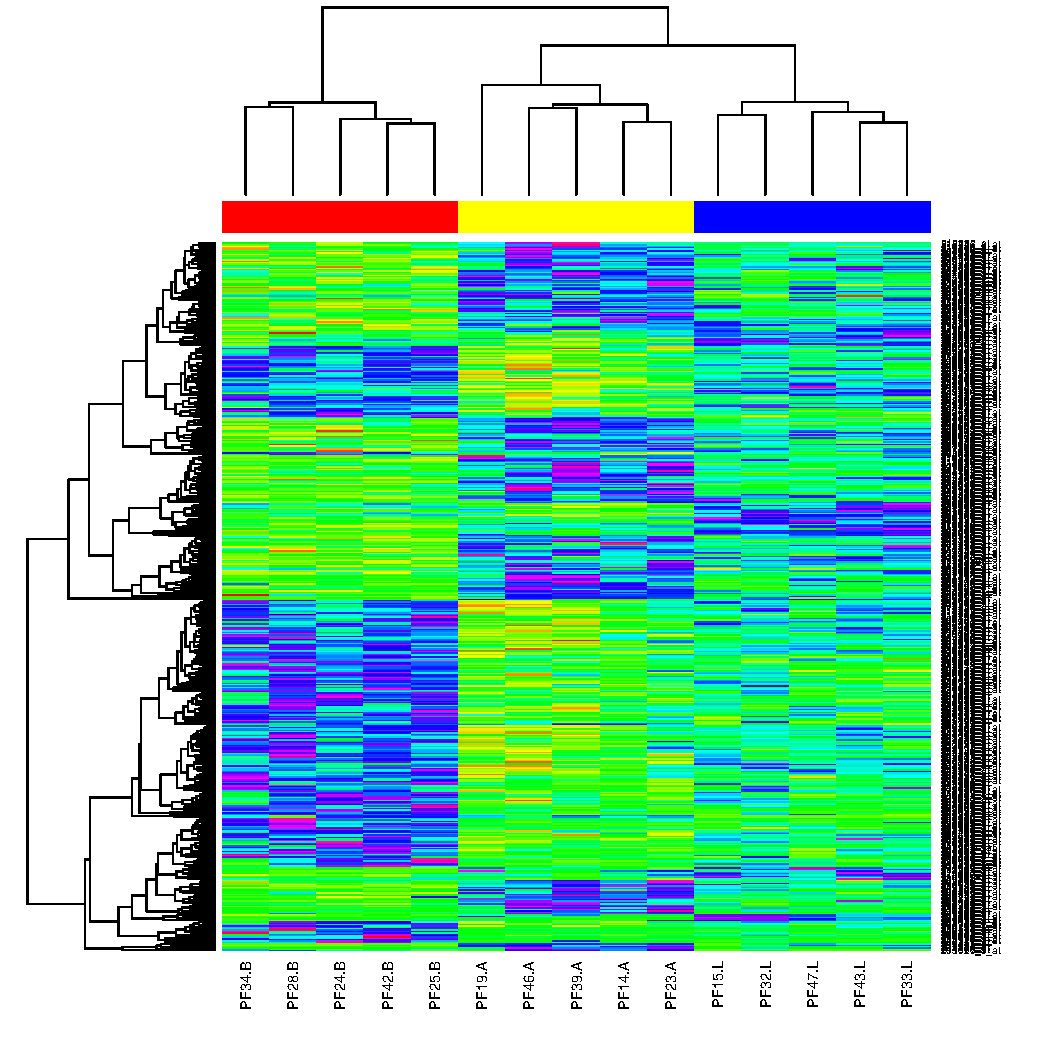
\includegraphics[width=\maxwidth]{images/graficplotHeatMap1-1} 

\end{knitrout}
\caption{Mapa de colores basado en los genes seleccionados por estar diferencialmente expresados. Como puede verse los tumores Apocrinos y Luminales tienen perfiles de expresión más parecidos entre ellos que cada uno con los de tipo Basal}
\label{fig:heatmap1}
\end{figure}

Si se desea realizar mapas de color más sofisticados puede utilizarse el paquete \Rpackage{gplots}
que implementa una version mejorada en la función \texttt{heatmap.2}


\begin{figure}[htbp]
\centering
\begin{knitrout}
\definecolor{shadecolor}{rgb}{0.969, 0.969, 0.969}\color{fgcolor}\begin{kframe}
\begin{alltt}
\hlstd{grupColors} \hlkwb{<-} \hlkwd{unlist}\hlstd{(}\hlkwd{lapply}\hlstd{(}\hlkwd{pData}\hlstd{(eset_rma)}\hlopt{$}\hlstd{Group, color.map))}
\hlkwd{require}\hlstd{(}\hlstr{"gplots"}\hlstd{)}
\hlkwd{heatmap.2}\hlstd{(exprs2cluster,}
          \hlkwc{col}\hlstd{=}\hlkwd{bluered}\hlstd{(}\hlnum{75}\hlstd{),} \hlkwc{scale}\hlstd{=}\hlstr{"row"}\hlstd{,}
          \hlkwc{ColSideColors}\hlstd{=grupColors,} \hlkwc{key}\hlstd{=}\hlnum{TRUE}\hlstd{,} \hlkwc{symkey}\hlstd{=}\hlnum{FALSE}\hlstd{,}
          \hlkwc{density.info}\hlstd{=}\hlstr{"none"}\hlstd{,} \hlkwc{trace}\hlstd{=}\hlstr{"none"}\hlstd{,} \hlkwc{cexCol}\hlstd{=}\hlnum{1}\hlstd{)}
\end{alltt}
\end{kframe}
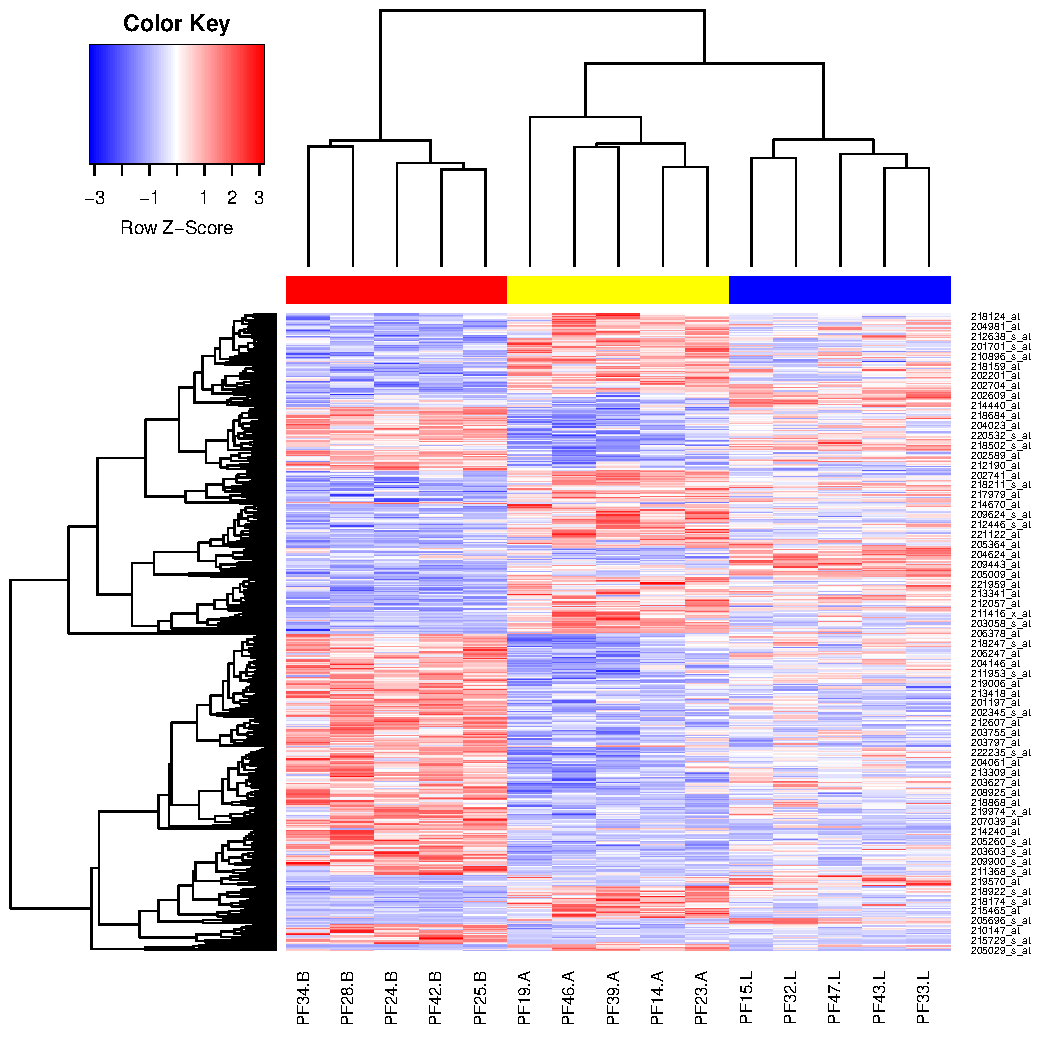
\includegraphics[width=\maxwidth]{images/graficplotHeatMap2-1} 

\end{knitrout}
\caption{Mapa de colores mejorado basado en los genes seleccionados por estar diferencialmente expresados. Como puede verse los tumores Apocrinos y Luminales tienen perfiles de expresión más parecidos entre ellos que cada uno con los de tipo Basal}
\label{fig:heatmap2}
\end{figure}

\subsection{Análisis de la significación biológica (1): Anàlisi de enriquecimiento}

El análisis de significación biológica busca establecer si, dada una lista de genes seleccionados por estar diferencialmente expresados entre dos condiciones, las funciones y procesos biológicos que los caracterizan aparecen en esta lista con mayor frecuencia que entre el resto de genes analizados.

Se han desarrollad multitud de variantes de estos tipos de análisis (\cite{Khatri:2005}) pero aquí utilizaremos el análisis básico de enriquecimiento tal como se describe en los trabajos de Gentleman (\cite{Gentleman:2004}) implementados en el paquete \texttt{GOstats} de Bioconductor.

El análisis se realiza sobre dos bases de datos de anotaciones, la "Gene Ontology'' o la ``Kyoto Encyclopedia of Genes and Genomes''.

Los análisis de este tipo necesitan un número mínimo de genes para resultar fiables por lo que se incluiran en todos los genes con p--valores ajustados inferiores a 0.05 (sin filtrar por minimo ``fold--change'').

\begin{knitrout}
\definecolor{shadecolor}{rgb}{0.969, 0.969, 0.969}\color{fgcolor}\begin{kframe}
\begin{alltt}
\hlkwd{require}\hlstd{(GOstats)}
\hlstd{listOfTables} \hlkwb{<-} \hlkwd{list}\hlstd{(}\hlkwc{AvsB} \hlstd{= topTab_AvsB,} \hlkwc{AvsL} \hlstd{= topTab_AvsL,} \hlkwc{BvsL} \hlstd{= topTab_BvsL)}
\hlkwa{for} \hlstd{(i} \hlkwa{in} \hlnum{1}\hlopt{:}\hlkwd{length}\hlstd{(listOfTables))\{}
  \hlcom{# Seleccionamos la "topTable"}
  \hlstd{topTab} \hlkwb{<-} \hlstd{listOfTables[[i]]}
  \hlcom{# Definimos el universo de genes: todos los que se han incluido en el análisis}
  \hlcom{# EL programa trabaja con identificadores "entrez" y no admite duplicados}

  \hlstd{entrezUniverse} \hlkwb{=} \hlkwd{unique}\hlstd{(}\hlkwd{getEG}\hlstd{(}\hlkwd{rownames}\hlstd{(topTab),} \hlstr{"hgu133a.db"}\hlstd{))}

  \hlcom{# Escogemos los grupos de sondas a incluir en el análisis}
  \hlcom{# Este análisis trabaja bien con varios centenares de genes }
  \hlcom{# por lo que es habitual basarse en p-valores sin ajustar para incluirlos}

  \hlstd{whichGenes}\hlkwb{<-}\hlstd{topTab[}\hlstr{"adj.P.Val"}\hlstd{]}\hlopt{<}\hlnum{0.05}
  \hlstd{geneIds} \hlkwb{<-}   \hlkwd{unique}\hlstd{(}\hlkwd{getEG}\hlstd{(}\hlkwd{rownames}\hlstd{(topTab)[whichGenes],}\hlstr{"hgu133a.db"}\hlstd{))}

  \hlcom{# Creamos los "hiperparámetros" en que se basa el análisis}
  \hlstd{GOparams} \hlkwb{=} \hlkwd{new}\hlstd{(}\hlstr{"GOHyperGParams"}\hlstd{,}
    \hlkwc{geneIds}\hlstd{=geneIds,} \hlkwc{universeGeneIds}\hlstd{=entrezUniverse,}
    \hlkwc{annotation}\hlstd{=}\hlstr{"org.Hs.eg.db"}\hlstd{,} \hlkwc{ontology}\hlstd{=}\hlstr{"BP"}\hlstd{,}
    \hlkwc{pvalueCutoff}\hlstd{=}\hlnum{0.001}\hlstd{,} \hlkwc{conditional}\hlstd{=}\hlnum{FALSE}\hlstd{,}
    \hlkwc{testDirection}\hlstd{=}\hlstr{"over"}\hlstd{)}
  \hlstd{KEGGparams} \hlkwb{=} \hlkwd{new}\hlstd{(}\hlstr{"KEGGHyperGParams"}\hlstd{,}
    \hlkwc{geneIds}\hlstd{=geneIds,} \hlkwc{universeGeneIds}\hlstd{=entrezUniverse,}
    \hlkwc{annotation}\hlstd{=}\hlstr{"org.Hs.eg.db"}\hlstd{,}
    \hlkwc{pvalueCutoff}\hlstd{=}\hlnum{0.01}\hlstd{,} \hlkwc{testDirection}\hlstd{=}\hlstr{"over"}\hlstd{)}

  \hlcom{# Ejecutamos los análisis}

  \hlstd{GOhyper} \hlkwb{=} \hlkwd{hyperGTest}\hlstd{(GOparams)}
  \hlstd{KEGGhyper} \hlkwb{=} \hlkwd{hyperGTest}\hlstd{(KEGGparams)}

\hlcom{# Creamos un informe html con los resultados}
   \hlstd{comparison} \hlkwb{=} \hlkwd{names}\hlstd{(listOfTables)[i]}
   \hlstd{GOfilename} \hlkwb{=}\hlkwd{file.path}\hlstd{(resultsDir,}
     \hlkwd{paste}\hlstd{(}\hlstr{"GOResults."}\hlstd{,comparison,}\hlstr{".html"}\hlstd{,} \hlkwc{sep}\hlstd{=}\hlstr{""}\hlstd{))}
   \hlstd{KEGGfilename} \hlkwb{=}\hlkwd{file.path}\hlstd{(resultsDir,}
     \hlkwd{paste}\hlstd{(}\hlstr{"KEGGResults."}\hlstd{,comparison,}\hlstr{".html"}\hlstd{,} \hlkwc{sep}\hlstd{=}\hlstr{""}\hlstd{))}
  \hlkwd{htmlReport}\hlstd{(GOhyper,} \hlkwc{file} \hlstd{= GOfilename,} \hlkwc{summary.args}\hlstd{=}\hlkwd{list}\hlstd{(}\hlstr{"htmlLinks"}\hlstd{=}\hlnum{TRUE}\hlstd{))}
  \hlkwd{htmlReport}\hlstd{(KEGGhyper,} \hlkwc{file} \hlstd{= KEGGfilename,} \hlkwc{summary.args}\hlstd{=}\hlkwd{list}\hlstd{(}\hlstr{"htmlLinks"}\hlstd{=}\hlnum{TRUE}\hlstd{))}
\hlstd{\}}
\end{alltt}
\end{kframe}
\end{knitrout}

\subsection{Análisis de la significación biológica (2): Expresión diferencial de conjuntos de genes}

El análisis de enriquecimiento adolece de un problema consistente en que parte de una lista de genes que ha sido truncada por un punto de corte más o menos arbitraria, lo que deja a muchos posibles genes interesantes fuera del análisis.

EL ``Gene Set Enrichment Analysis" fue introducido para intentar soslayar esta característica. La idea venía a ser que, aunque a veces un gen dado pudiera no estar diferencialmente expresado, un grupo de genes relacionado con una característica médica (enfermedad) o biológica (proceso) podría tender a mostrar más diferencias entre los grupos en estudio que el resto de los genes. Es decir aunque gen a gen no hubiera expresión diferencial este método podría detectars diferencias a nivel del grupo de genes.

A partir del método original se han desarrollado múltiples variaciones. 
Aquí presentamos la propuesta por Efronn y Tibshirani.

Este método necesita
\begin{itemize}
  \item Una matriz de expresión, con una fila por gen, y una columna por muestra
  \item Un vector de condiciones experimentales
  \item Un vector de nombres de los genes
  \item Una lista de grupos de genes (``genesets'')
\end{itemize}

Por simplicidad se analizará la primera comparaci\'on: ``A vs B''.

\begin{knitrout}
\definecolor{shadecolor}{rgb}{0.969, 0.969, 0.969}\color{fgcolor}\begin{kframe}
\begin{alltt}
\hlkwd{require}\hlstd{(annotate)}
\hlkwd{require}\hlstd{(hgu133plus2.db)}
\end{alltt}


{\ttfamily\noindent\itshape\color{messagecolor}{\#\# Loading required package: hgu133plus2.db}}

{\ttfamily\noindent\itshape\color{messagecolor}{\#\# }}\begin{alltt}
\hlstd{geneSets} \hlkwb{<-} \hlkwd{read.csv}\hlstd{(}\hlkwd{file.path}\hlstd{(dataDir,} \hlstr{"PBTs_all_affy.csv"}\hlstd{))}

\hlcom{## gene sets a comparar amb cadascuna de les toptable}
\hlstd{gsEntrez} \hlkwb{<-} \hlkwd{list}\hlstd{()}
\hlkwa{for} \hlstd{(i} \hlkwa{in} \hlnum{1}\hlopt{:}\hlkwd{dim}\hlstd{(geneSets)[}\hlnum{2}\hlstd{]) \{}
  \hlstd{gs} \hlkwb{<-} \hlkwd{as.character}\hlstd{(geneSets[,i])}
  \hlstd{gs} \hlkwb{<-} \hlstd{gs[gs} \hlopt{!=} \hlstr{""}\hlstd{]}
  \hlstd{gsE} \hlkwb{<-} \hlkwd{getEG}\hlstd{(gs,} \hlkwc{data} \hlstd{=} \hlstr{"hgu133plus2.db"}\hlstd{)}
  \hlstd{gsEntrez[[}\hlkwd{colnames}\hlstd{(geneSets[i])]]} \hlkwb{<-} \hlkwd{unique}\hlstd{(gsE[}\hlopt{!}\hlkwd{is.na}\hlstd{(gsE)])}
\hlstd{\}}

\hlstd{gsSymbol} \hlkwb{<-} \hlkwd{list}\hlstd{()}
\hlkwa{for} \hlstd{(i} \hlkwa{in} \hlnum{1}\hlopt{:}\hlkwd{dim}\hlstd{(geneSets)[}\hlnum{2}\hlstd{]) \{}
  \hlstd{gs} \hlkwb{<-} \hlkwd{as.character}\hlstd{(geneSets[,i])}
  \hlstd{gs} \hlkwb{<-} \hlstd{gs[gs} \hlopt{!=} \hlstr{""}\hlstd{]}
  \hlstd{gsSymb} \hlkwb{<-} \hlkwd{getSYMBOL}\hlstd{(gs,}\hlkwc{data} \hlstd{=} \hlstr{"hgu133plus2.db"}\hlstd{)}
  \hlstd{gsSymbol[[}\hlkwd{colnames}\hlstd{(geneSets[i])]]} \hlkwb{<-} \hlkwd{unique}\hlstd{(gsSymb[}\hlopt{!}\hlkwd{is.na}\hlstd{(gsSymb)])}
\hlstd{\}}
\hlstd{genesetsNames} \hlkwb{<-} \hlkwd{names}\hlstd{(gsEntrez)}
\end{alltt}
\end{kframe}
\end{knitrout}


\begin{knitrout}
\definecolor{shadecolor}{rgb}{0.969, 0.969, 0.969}\color{fgcolor}\begin{kframe}
\begin{alltt}
\hlkwd{require}\hlstd{(genefilter)}
\hlstd{esetUnique} \hlkwb{<-} \hlkwd{featureFilter}\hlstd{(eset_rma,} \hlkwc{require.entrez}\hlstd{=}\hlnum{TRUE}\hlstd{,} \hlkwc{remove.dupEntrez}\hlstd{=}\hlnum{FALSE}\hlstd{)}
\hlkwd{dim}\hlstd{(}\hlkwd{exprs}\hlstd{(esetUnique))}
\end{alltt}
\begin{verbatim}
## [1] 19845    15
\end{verbatim}
\begin{alltt}
\hlstd{esetUnique} \hlkwb{<-} \hlkwd{featureFilter}\hlstd{(eset_rma,} \hlkwc{require.entrez}\hlstd{=}\hlnum{TRUE}\hlstd{,} \hlkwc{remove.dupEntrez}\hlstd{=}\hlnum{TRUE}\hlstd{)}
\hlkwd{dim}\hlstd{(}\hlkwd{exprs}\hlstd{(esetUnique))}
\end{alltt}
\begin{verbatim}
## [1] 12437    15
\end{verbatim}
\begin{alltt}
\hlstd{esetAB}\hlkwb{<-} \hlstd{esetUnique[,}\hlkwd{pData}\hlstd{(esetUnique)}\hlopt{$}\hlstd{Group} \hlopt \hlkwd{c}\hlstd{(}\hlstr{"A"}\hlstd{,}\hlstr{"B"}\hlstd{)]}
\hlkwd{pData}\hlstd{(esetAB)}
\end{alltt}
\begin{verbatim}
##                Sample             Ids SampleIDs Group Apocrine.grade
## GSM26878.CEL GSM26878 PF14 EnPnT2N1G2      PF14     A              3
## GSM26883.CEL GSM26883 PF19 EnPuT4N0Gu      PF19     A              2
## GSM26887.CEL GSM26887 PF23 EnPnT2N0G2      PF23     A              3
## GSM26903.CEL GSM26903 PF39 EnPuT4N0Gu      PF39     A              3
## GSM26910.CEL GSM26910 PF46 EnPnT4N1G3      PF46     A              3
## GSM26888.CEL GSM26888 PF24 EnPnTiN0G3      PF24     B              2
## GSM26889.CEL GSM26889 PF25 EnPnT3N2G2      PF25     B              1
## GSM26892.CEL GSM26892 PF28 EnPnT2N1G3      PF28     B              2
## GSM26898.CEL GSM26898 PF34 EnPnT3N1G3      PF34     B              1
## GSM26906.CEL GSM26906 PF42 EnPnT2N2G3      PF42     B             na
##              AR.repeat.length
## GSM26878.CEL               18
## GSM26883.CEL               18
## GSM26887.CEL               18
## GSM26903.CEL               17
## GSM26910.CEL               19
## GSM26888.CEL               NA
## GSM26889.CEL               21
## GSM26892.CEL               22
## GSM26898.CEL               17
## GSM26906.CEL               16
\end{verbatim}
\begin{alltt}
\hlstd{xAB} \hlkwb{<-} \hlkwd{exprs}\hlstd{(esetAB)}
\hlstd{yAB} \hlkwb{<-} \hlkwd{ifelse}\hlstd{(}\hlkwd{pData}\hlstd{(esetAB)}\hlopt{$}\hlstd{Group}\hlopt{==}\hlstr{"A"}\hlstd{,} \hlnum{1}\hlstd{,} \hlnum{2}\hlstd{)}
\hlstd{entrezs}\hlkwb{<-}\hlkwd{getEG}\hlstd{(}\hlkwd{rownames}\hlstd{(xAB),} \hlstr{"hgu133a"}\hlstd{)}
\hlstd{simbols} \hlkwb{<-}\hlkwd{getSYMBOL}\hlstd{(}\hlkwd{rownames}\hlstd{(xAB),} \hlstr{"hgu133a"}\hlstd{)}
\end{alltt}
\end{kframe}
\end{knitrout}

Una vez recopilados los componentes necesarios se ejecuta la llamada al método \texttt{GSA}

\begin{knitrout}
\definecolor{shadecolor}{rgb}{0.969, 0.969, 0.969}\color{fgcolor}\begin{kframe}
\begin{alltt}
\hlkwd{require}\hlstd{(GSA)}
\hlstd{GSA.obj}\hlkwb{<-}\hlkwd{GSA}\hlstd{(xAB, yAB,} \hlkwc{genenames}\hlstd{=entrezs,} \hlkwc{genesets}\hlstd{=gsEntrez,}  \hlkwc{resp.type}\hlstd{=}\hlstr{"Two class unpaired"}\hlstd{,} \hlkwc{nperms}\hlstd{=}\hlnum{100}\hlstd{)}
\end{alltt}
\begin{verbatim}
## perm= 10 / 100 
## perm= 20 / 100 
## perm= 30 / 100 
## perm= 40 / 100 
## perm= 50 / 100 
## perm= 60 / 100 
## perm= 70 / 100 
## perm= 80 / 100 
## perm= 90 / 100 
## perm= 100 / 100
\end{verbatim}
\begin{alltt}
\hlkwd{GSA.listsets}\hlstd{(GSA.obj,} \hlkwc{geneset.names}\hlstd{=genesetsNames,} \hlkwc{FDRcut}\hlstd{=}\hlnum{.5}\hlstd{)}
\end{alltt}
\begin{verbatim}
## $FDRcut
## [1] 0.5
## 
## $negative
##      Gene_set Gene_set_name Score     p-value FDR    
## [1,] "17"     "KT1.1"       "-0.8933" "0"     "0"    
## [2,] "16"     "KT2"         "-0.6307" "0.05"  "0.325"
## [3,] "18"     "KT2.1"       "-0.6559" "0.09"  "0.39" 
## 
## $positive
##      Gene_set Gene_set_name Score p-value FDR
## 
## $nsets.neg
## [1] 3
## 
## $nsets.pos
## [1] 0
\end{verbatim}
\end{kframe}
\end{knitrout}

Si en vez de usar una lista ``ad-hoc" de genesets se desea utilizar conjuntos públicos, pueden descargarse de sitios como el Broad Institute \url{http://software.broadinstitute.org/gsea/downloads.jsp} en formato \texttt{.gmt}.

En este ejemplo se utiliza el conjunto de grupos de genes definidos por los pathways de KEGG.

\begin{knitrout}
\definecolor{shadecolor}{rgb}{0.969, 0.969, 0.969}\color{fgcolor}\begin{kframe}
\begin{alltt}
\hlstd{geneset.obj} \hlkwb{<-} \hlkwd{GSA.read.gmt}\hlstd{(}\hlkwd{file.path}\hlstd{(dataDir,}\hlstr{"c2.cp.kegg.v5.1.entrez.gmt"}\hlstd{))}
\end{alltt}
\begin{verbatim}
## 1234567891011121314151617181920212223242526272829303132333435363738394041424344454647484950515253545556575859606162636465666768697071727374757677787980818283848586878889909192939495969798991001011021031041051061071081091101111121131141151161171181191201211221231241251261271281291301311321331341351361371381391401411421431441451461471481491501511521531541551561571581591601611621631641651661671681691701711721731741751761771781791801811821831841851861
## 2
## 3
## 4
## 5
## 6
## 7
## 8
## 9
## 10
## 11
## 12
## 13
## 14
## 15
## 16
## 17
## 18
## 19
## 20
## 21
## 22
## 23
## 24
## 25
## 26
## 27
## 28
## 29
## 30
## 31
## 32
## 33
## 34
## 35
## 36
## 37
## 38
## 39
## 40
## 41
## 42
## 43
## 44
## 45
## 46
## 47
## 48
## 49
## 50
## 51
## 52
## 53
## 54
## 55
## 56
## 57
## 58
## 59
## 60
## 61
## 62
## 63
## 64
## 65
## 66
## 67
## 68
## 69
## 70
## 71
## 72
## 73
## 74
## 75
## 76
## 77
## 78
## 79
## 80
## 81
## 82
## 83
## 84
## 85
## 86
## 87
## 88
## 89
## 90
## 91
## 92
## 93
## 94
## 95
## 96
## 97
## 98
## 99
## 100
## 101
## 102
## 103
## 104
## 105
## 106
## 107
## 108
## 109
## 110
## 111
## 112
## 113
## 114
## 115
## 116
## 117
## 118
## 119
## 120
## 121
## 122
## 123
## 124
## 125
## 126
## 127
## 128
## 129
## 130
## 131
## 132
## 133
## 134
## 135
## 136
## 137
## 138
## 139
## 140
## 141
## 142
## 143
## 144
## 145
## 146
## 147
## 148
## 149
## 150
## 151
## 152
## 153
## 154
## 155
## 156
## 157
## 158
## 159
## 160
## 161
## 162
## 163
## 164
## 165
## 166
## 167
## 168
## 169
## 170
## 171
## 172
## 173
## 174
## 175
## 176
## 177
## 178
## 179
## 180
## 181
## 182
## 183
## 184
## 185
\end{verbatim}
\begin{alltt}
\hlstd{GSA.obj2} \hlkwb{<-} \hlkwd{GSA}\hlstd{(xAB, yAB,} \hlkwc{genenames}\hlstd{=entrezs,} \hlkwc{genesets}\hlstd{=geneset.obj}\hlopt{$}\hlstd{genesets,}  \hlkwc{resp.type}\hlstd{=}\hlstr{"Two class unpaired"}\hlstd{,} \hlkwc{nperms}\hlstd{=}\hlnum{100}\hlstd{)}
\end{alltt}
\begin{verbatim}
## perm= 10 / 100 
## perm= 20 / 100 
## perm= 30 / 100 
## perm= 40 / 100 
## perm= 50 / 100 
## perm= 60 / 100 
## perm= 70 / 100 
## perm= 80 / 100 
## perm= 90 / 100 
## perm= 100 / 100
\end{verbatim}
\begin{alltt}
\hlkwd{GSA.listsets} \hlstd{(GSA.obj2,} \hlkwc{geneset.names}\hlstd{=geneset.obj}\hlopt{$}\hlstd{geneset.names,} \hlkwc{FDRcut}\hlstd{=}\hlnum{.5}\hlstd{)}
\end{alltt}
\begin{verbatim}
## $FDRcut
## [1] 0.5
## 
## $negative
##       Gene_set Gene_set_name          Score     p-value FDR     
##  [1,] "4"      "KEGG_PENTOSE_AND_GLU" "-1.0474" "0"     "0"     
##  [2,] "7"      "KEGG_ASCORBATE_AND_A" "-1.1019" "0"     "0"     
##  [3,] "23"     "KEGG_TYROSINE_METABO" "-0.6995" "0"     "0"     
##  [4,] "33"     "KEGG_O_GLYCAN_BIOSYN" "-0.6857" "0"     "0"     
##  [5,] "69"     "KEGG_DRUG_METABOLISM" "-0.5306" "0"     "0"     
##  [6,] "142"    "KEGG_INSULIN_SIGNALI" "-0.3796" "0"     "0"     
##  [7,] "11"     "KEGG_STEROID_HORMONE" "-0.7588" "0.01"  "0.178" 
##  [8,] "30"     "KEGG_STARCH_AND_SUCR" "-0.3887" "0.01"  "0.178" 
##  [9,] "67"     "KEGG_METABOLISM_OF_X" "-0.6237" "0.01"  "0.178" 
## [10,] "68"     "KEGG_DRUG_METABOLISM" "-0.5961" "0.01"  "0.178" 
## [11,] "62"     "KEGG_TERPENOID_BACKB" "-0.7314" "0.02"  "0.2967"
## [12,] "102"    "KEGG_MTOR_SIGNALING_" "-0.3444" "0.02"  "0.2967"
## [13,] "60"     "KEGG_RETINOL_METABOL" "-0.5196" "0.03"  "0.356" 
## [14,] "87"     "KEGG_ERBB_SIGNALING_" "-0.237"  "0.03"  "0.356" 
## [15,] "10"     "KEGG_PRIMARY_BILE_AC" "-0.5234" "0.04"  "0.356" 
## [16,] "29"     "KEGG_GLUTATHIONE_MET" "-0.4147" "0.04"  "0.356" 
## [17,] "39"     "KEGG_GLYCEROLIPID_ME" "-0.4147" "0.04"  "0.356" 
## [18,] "91"     "KEGG_PHOSPHATIDYLINO" "-0.2111" "0.04"  "0.356" 
## [19,] "101"    "KEGG_PEROXISOME"      "-0.7756" "0.04"  "0.356" 
## [20,] "166"    "KEGG_ENDOMETRIAL_CAN" "-0.3821" "0.04"  "0.356" 
## [21,] "16"     "KEGG_GLYCINE_SERINE_" "-0.3191" "0.05"  "0.387" 
## [22,] "80"     "KEGG_PPAR_SIGNALING_" "-0.46"   "0.05"  "0.387" 
## [23,] "146"    "KEGG_ADIPOCYTOKINE_S" "-0.2582" "0.05"  "0.387" 
## 
## $positive
##      Gene_set Gene_set_name Score p-value FDR
## 
## $nsets.neg
## [1] 23
## 
## $nsets.pos
## [1] 0
\end{verbatim}
\end{kframe}
\end{knitrout}

\section{Resumen de resultados y discusión}

Los controles de calidad llevados a cabo en la primera parte de  este estudio han permitido establecer que los datos con los que se ha trabajado eran de buena calidad, a pesar de presentar una cierta heterogeneidad que queda ilustrada en la incompleta agrupación de las muestras segun sus tipos de tumores.

Los análisis llevados a cabo sobre los datos normalizados y filtrados han permitido detectar un cierto número de genes diferencialmente expresados (ver tabla \ref{resum1}) que se prestan a estudios posteriores acerca de su significación biológica.

\begin{table}[htbp]
\caption{Genes diferencialmente expresados basados en un cirte definido por un p-valor ajustado (FDR) inferior a 0.05 y un cambio de expresión de cómo mínimo 1.}
\begin{tabular}{|l|c|c|c|}
\hline
 & A vs B & A vs L & B vs L \\ \hline
Genes “down-regulados” & 228 & 29 & 113 \\ \hline
Genes “sobre-expresados” & 174 & 27 & 111 \\ \hline
\end{tabular}
\label{resum1}
\end{table}

La lista completas de genes seleccionados (ordenados de mayor a menor p--valor) pueden verse en los archivos ``Selected genes in comparison AvsB.html'', ``Selected genes in comparison AvsL.html'' y ``Selected genes in comparison BvsL.html''.

El análisis de significación biológica ha permitido detectar una serie de funciones y procesos biológicos que caracterizan las listas de genes seleccionadas en las bases de datos de anotaciones más populares, la Gene Ontology (GO) y la ``Kyoto Enyclopedia of Genes and Genomes''. Estas listas pueden verse en las tablas ``GOResults.XXvsYY.html'' y ``KEGGResults.XXvsYY.html'' (XXvsYY es AvsB, AvsL o BvsL) pero no se discuten aquí.

\subsection{Discusión}

El estudio que se ha presentado en este documento es un análisis estándar de microarrays y como tal adolece de sus ventajas e inconvenientes.

Como inconveniente podemos destacar dos cosas
\begin{itemize}
\item El tamaño de las muestras utilizadas es bastante limitado lo que determina que el estudio tenga poca potencia por lo que \emph{probablemente} habrá menos reproducibilidad y más falsos negativos de los que sería deseable si se utilizara un mayor número de muestras.
\item En cada paso del proceso se han tomado decisiones relativamente arbitrarias acerca de los métodos a seguir para la normalización, filtradom selección de genes, etc. La decisión de si estos métodos son los más adecuados o no es probablemente subjetiva (véase por ejemplo los artículos ~\cite{Choe:2005, Zhu:2010}) por lo que sería interesante saber como cambian los resultados si se tomaran otras decisiones.
\end{itemize}

Los problemas anteriores no son, sin embargo, problemas de este estudio concreto, sino en general de los estudios basados en microarrays por lo que, limitaciones aparte, el estudio aportará probablemente información valiosa que permitirá un seguimiento posterior del problema.

Finalmente debe de tenerse en cuenta que cualquier gen que se acabe considerando realmente expresado diferencialmente se tendrá que verificar mediante otras técnicas como RT-qPCR por lo que este estudio debe de considerarse como un paso hacia el descubrimiento de genes candidatos, no como una fase definitiva.


%\subsubsection{Tablas de resultados}
%Un análisis como el que se ha realizado en este ejercicio genera una gran cantidad de archivos de resultados. \emph{Una buena práctica} en estos casos es preparar algun tipo de tabla que permita tener una visión panorámica de los resultados o navegar entre ellos.
%Esto puede hacers de forma relativamente sencilla con el paquete \texttt{hwriter}

\bibliography{MDA-references}

\appendix{Codigo R del análisis}

El archivo \texttt{EjemploAnalisisMicroarrays.R} contiene el código R utilizado para realizar todos los análisis presentados en este informe.

El análisis se ha llevado a cabo utilizando el sistema \texttt{Sweave} (\cite{Leisch:2002a, Leisch:2002b}) de análisis reproducibles que integra el sistema \LaTeX y el lenguaje \R para generar a la vez los análisis y el informe de resultados por lo que el código puede contener alguna instrucción inusual cuando su objetivo es generar una tabla de \LaTeX. Aparte de ésto es un código estándar en el que se ha procurado no usar funciones avanzadas sino básicamente lo que se ha discutido en el curso.

\end{document}

\appendix{Lista de archivos generados en el estudio}

La tabla \ref{listaArchivos} contiene una lista de los archivos generados en este estudio. 

\begin{kframe}


{\ttfamily\noindent\itshape\color{messagecolor}{\#\# Loading required package: gdata}}

{\ttfamily\noindent\itshape\color{messagecolor}{\#\# gdata: read.xls support for 'XLS' (Excel 97-2004) files ENABLED.}}

{\ttfamily\noindent\itshape\color{messagecolor}{\#\# }}

{\ttfamily\noindent\itshape\color{messagecolor}{\#\# gdata: Unable to load perl libaries needed by read.xls()\\\#\# gdata: to support 'XLSX' (Excel 2007+) files.}}

{\ttfamily\noindent\itshape\color{messagecolor}{\#\# }}

{\ttfamily\noindent\itshape\color{messagecolor}{\#\# gdata: Run the function 'installXLSXsupport()'\\\#\# gdata: to automatically download and install the perl\\\#\# gdata: libaries needed to support Excel XLS and XLSX formats.}}

{\ttfamily\noindent\itshape\color{messagecolor}{\#\# \\\#\# Attaching package: 'gdata'}}

{\ttfamily\noindent\itshape\color{messagecolor}{\#\# The following object is masked from 'package:IRanges':\\\#\# \\\#\#\ \ \ \  trim}}

{\ttfamily\noindent\itshape\color{messagecolor}{\#\# The following object is masked from 'package:S4Vectors':\\\#\# \\\#\#\ \ \ \  first}}

{\ttfamily\noindent\itshape\color{messagecolor}{\#\# The following object is masked from 'package:stats4':\\\#\# \\\#\#\ \ \ \  nobs}}

{\ttfamily\noindent\itshape\color{messagecolor}{\#\# The following object is masked from 'package:Biobase':\\\#\# \\\#\#\ \ \ \  combine}}

{\ttfamily\noindent\itshape\color{messagecolor}{\#\# The following object is masked from 'package:BiocGenerics':\\\#\# \\\#\#\ \ \ \  combine}}

{\ttfamily\noindent\itshape\color{messagecolor}{\#\# The following object is masked from 'package:stats':\\\#\# \\\#\#\ \ \ \  nobs}}

{\ttfamily\noindent\itshape\color{messagecolor}{\#\# The following object is masked from 'package:utils':\\\#\# \\\#\#\ \ \ \  object.size}}

{\ttfamily\noindent\itshape\color{messagecolor}{\#\# The following object is masked from 'package:base':\\\#\# \\\#\#\ \ \ \  startsWith}}\end{kframe}                            listaArchivos
1                         anotations.html
2                            arrayQuality
3                      AvsB.EntrezAll.csv
4                 AvsB.EntrezSelected.csv
5                AvsB.SymbolsSelected.csv
6                      AvsL.EntrezAll.csv
7                 AvsL.EntrezSelected.csv
8                AvsL.SymbolsSelected.csv
9                      BvsL.EntrezAll.csv
10                BvsL.EntrezSelected.csv
11               BvsL.SymbolsSelected.csv
12                 Datos.Normalizados.csv
13                Datos.Normalizados.csv2
14      Datos.Normalizados.Filtrados.csv2
15                 datos.normalizados.Rda
16                 ExpressAndTop.AvsB.ods
17                 ExpressAndTop.AvsL.ods
18                 ExpressAndTop.BvsL.ods
19                ExpressAndTop_AvsB.csv2
20                ExpressAndTop_AvsL.csv2
21                ExpressAndTop_BvsL.csv2
22                    GOResults.AvsB.html
23                    GOResults.AvsL.html
24                    GOResults.BvsL.html
25                  KEGGResults.AvsB.html
26                  KEGGResults.AvsL.html
27                  KEGGResults.BvsL.html
28                     listaArchivos.html
29 Selected Genes in comparison AvsB.html
30 Selected Genes in comparison AvsL.html
31 Selected Genes in comparison BvsL.html


Utilizando el paquete \texttt{hwriter} es posible generar de forma sencilla una tabla html con hiperenlaces que permita acceder a los distintos archivos generados en el análisis.


